\documentclass[11pt]{article}
\usepackage[utf8]{inputenc}
\usepackage{amsmath}
\usepackage{graphicx}
\usepackage{listings}
\usepackage{verbatim}
\usepackage{float}
\usepackage{xcolor}
\usepackage{subcaption}
\usepackage[english]{babel}
\usepackage{caption}
\usepackage{hyperref}
\usepackage{biblatex}
\addbibresource{project3.bib}
\usepackage{setspace}
\usepackage{wrapfig}
\usepackage{lipsum}
\usepackage{amssymb}
\linespread{1.15}
\usepackage[a4paper, total={6.5in, 9in}]{geometry}


\hypersetup{
    colorlinks,
    linkcolor={red!50!black},
    citecolor={blue!50!black},
    urlcolor={blue!80!black}
}
\definecolor{codegreen}{rgb}{0,0.6,0}
\definecolor{codegray}{rgb}{0.5,0.5,0.5}
\definecolor{codepurple}{rgb}{0.58,0,0.82}
\definecolor{backcolour}{rgb}{0.95,0.95,0.92}
\definecolor{dkgreen}{rgb}{0,0.6,0}
\definecolor{gray}{rgb}{0.5,0.5,0.5}
\definecolor{mauve}{rgb}{0.58,0,0.82}

\lstdefinestyle{mystyle}{
    backgroundcolor=\color{backcolour},
    commentstyle=\color{codegreen},
    keywordstyle=\color{magenta},
    numberstyle=\tiny\color{codegray},
    stringstyle=\color{codepurple},
    basicstyle=\ttfamily\footnotesize,
    breakatwhitespace=false,
    breaklines=true,
    captionpos=b,
    keepspaces=true,
    numbers=left,
    numbersep=5pt,
    showspaces=false,
    showstringspaces=false,
    showtabs=false,
    tabsize=2
}

\lstset{style=mystyle}
\title{Project 3\\ }
\author{Filip Severin von der Lippe}
\date{\today}
\begin{document}
\maketitle
GitHub repository containing code and further instructions on how to reproduce the results of this article: \url{https://github.com/Fslippe/FYS-STK4155/tree/main/project3}
\url{https://openarchive.usn.no/usn-xmlui/handle/11250/2581934}
\url{https://www.kaggle.com/datasets/jsphyg/weather-dataset-rattle-package}
\begin{abstract}
\end{abstract}
\newpage
\tableofcontents
\newpage
\section{Introduction}
The weather is a big part of our lives. It is something we all have a relationship with and have to consider in the planning of our daily lives. Precipitation is maybe what is most important for us to know about. It may make a day at the beach either a joyful or a not so enjoyable experience. This makes weather forecasts and their quality of importance in our daily planning. A possibility to improve the weather forecasts is by using machine learning methods. To test the use of such methods we will in this article use daily weather data from numerous Australian weather station from the time frame 2007 to 2017, to predict rain the next day. We will implement and compare logistic regression, a Feed Forward Neural Network and Random Forest and look at their performance when training on different data subsets. We will look into the methods' abilities of predicting rain at other locations than they have been trained at, and try finding the usefulness of the models in weather forecasting.

The article is structured in four main parts and an appendix. First we will introduce the data structure and the implementation of the methods in section \ref{sec:Method}, before presenting the results in section \ref{sec:Results}. We will discuss the results, and look at weaknesses and possibilities for improvements in the discussion section \ref{sec:Discussion}, before summarizing our findings in the conclusion in section \ref{sec:Conclusion}.
\section{Method}
\label{sec:Method}

\subsection{Structure of dataset} % (fold)

The dataset found on \href{https://www.kaggle.com/datasets/jsphyg/weather-dataset-rattle-package}{kaggle} includes about 10 years of weather observations from numerous Australian weather stations. The observations include features such as temperature, wind, rainfall, and sunshine hours. A full overview of the dataset and its features can be found in table \ref{tab:features} in appendix \ref{app:dataset}. The main purpose of the dataset is to make a prediction based on today's weather if it is going to rain or not tomorrow. This prediction is either Yes or No, and we are therefore looking at a binary classification problem.



\subsection{Initializing of dataset}
The initializing and importing of the datasets require a few steps before we can train our models. These include importing the dataset to a pandas dataframe and removing all rows (days) which has at least one measurement missing. This allows for an easy way to load a training set to our models by excluding Not a Number (NaN) values and their possible negative influence on our models. This leaves us with less data to work with, but still a large amount.

The dataset comes with wind directions given in a 16-wind compass rose as seen in figure \ref{fig:compass}. This may cause some problems for some neural networks or other methods not built to handle letters or words as input. To solve this problem we translate them to labels from 0 to 15 going clockwise from North (0) to North North-West (15) as seen in table \ref{tab:compass}. The location of the weather station is given in names which also may cause problems for some models. This is solved by restricting each train and test sample to either a specific weather station or specific indexes corresponding to certain locations.
\begin{figure}[H]
    \centering
    
\includegraphics[width=.3\textwidth]{../figures/Brosen_windrose.png}
    \caption{16-wind compass rose used to describe wind directions. Labels are defined as N (North), S (South), W (West) and E (East).}
    \label{fig:compass}
\end{figure}
\begin{table}[H]
    \begin{small}
        \caption{Translation and labeling of the different wind directions into integers from 0 to 15.}
        \label{tab:compass}
        \begin{center}
            \begin{tabular}{|c|c|c|c|c|c|c|c|c|c|c|c|c|c|c|c|}
                \hline
                N & NNE & NE & ENE & E & ESE & SE & SSE & S & SSW & SW & WSW & W  & WNW & NW & NNW \\
                \hline
                0 & 1   & 2  & 3   & 4 & 5   & 6  & 7   & 8 & 9   & 10 & 11  & 12 & 13  & 14 & 15  \\
                \hline
            \end{tabular}
        \end{center}
    \end{small}
\end{table}

\subsection{Choosing data to analyze} % (fold)
\label{sub:Weather stations}
For our testing of the models and the dataset we start by looking at one single weather station Cobar. The data from this weather station containts 534 days which makes it one of the smaller datasets, enabling fast testing of our model. For further analysis we mainly look into three different weather stations. The choices are based on geographic position in hopes of finding a trained model's location dependency as well as its flexibility. We again look at the station Cobar, the station Coffs Harbour slightly to the east, and the north most weather station Darwin. These locations are highlighted below in figure \ref{fig:earth}. We also look into the dataset as a whole combining all the weather stations marked in figure \ref{fig:earth}
\begin{figure}[H]
    \centering
    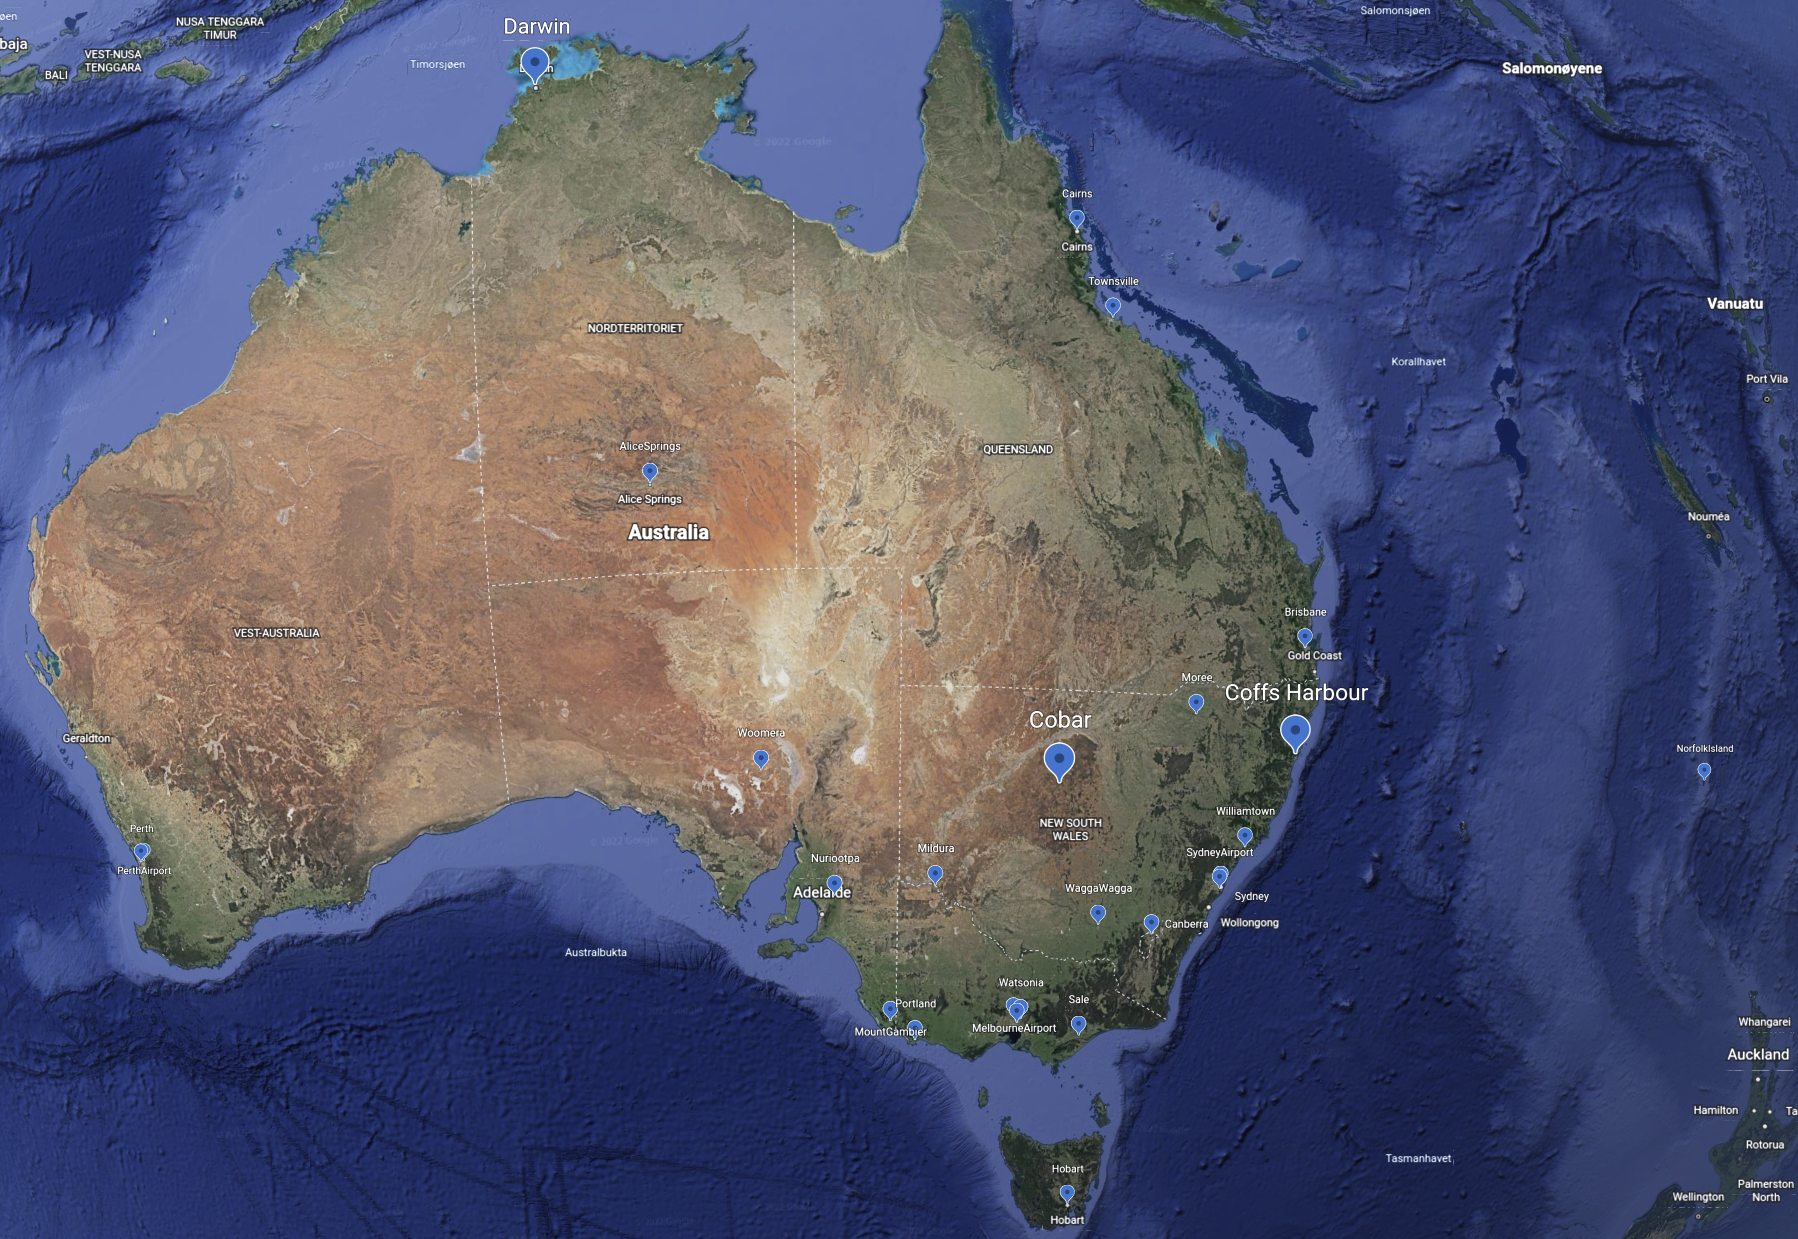
\includegraphics[width=\textwidth]{../figures/earth.png}
    \caption{Satellite image of Australia with all weather stations marked with blue points. The three stations Cobar, Darwin and Coffs Harbour which we will focus on are marked with larger points. \textit{Picture source: Screenshot from Google Earth dated 12. Dec. 2022.}}
    \label{fig:earth}
\end{figure}
% subsubsection Weather stations (end)

\subsection{Scaling and splitting the dataset}
To prepare our data for analysis we first scale the input data. We have chosen to use a standard scaler which reduces the mean to 0 and the variance to 1 for every feature of the data. This can be written for the data $x$ in terms of its mean $\overline{x}$ and standard deviation $\sigma_x$ as
\begin{align*}
    x_{scaled} = \frac{x - \overline{x}}{\sigma_x}.
\end{align*}
To reduce overfitting we perform a train-test split of our data. This is done by splitting the data in two subsets with 80\% in the train subset and 20\% in the test subset. By training our models on the train data, and optimizing them to give the highest possible accuracy on test data, our models become more generalized meaning they will not only perform well on the train data.

\subsection{Implementation of methods} % (fold)

\begin{table}[H]
    \begin{small}
        \caption{Notation used with descriptions and dimensions. }
        \label{tab:}
        \begin{center}
            \begin{tabular}{|l|l|l|}
                \hline
                Notation       & Description                                               & size                                \\
                \hline
                $C$            & Cost function                                             & -                                   \\
                \hline
                $\sigma$       & Activation function                                       & -                                   \\
                \hline
                $w_{ij}^{(L)}$ & The weight for the connection                             &                                     \\                     & between neuron $i$ in layer $L-1$   and $j$ in layer $L$ & - \\
                \hline
                $b_j^{(L)}$    & Bias added for neuron $j$ in layer $L$                    & -                                   \\
                \hline
                $z_j^{(L)}$    & Output before activation for neuron $j$ in layer $L$      & -                                   \\
                \hline
                $a_j^{(L)}$    & Output of activation function for neuron $j$ in layer $L$ & -                                   \\
                \hline
                $\lambda$      & L2-norm                                                   & -                                   \\
                \hline
                $B_k$          & Containing samples of minibatch $k$                       & -                                   \\
                \hline
                $M$            & The number of minibatches                                 & -                                   \\
                \hline
                $\eta_j$       & Step size (learning rate) at step $j$                     & $n$ iterations                      \\
                \hline
                $\theta$       & Value to optimize in our models                           & $n$ features                        \\
                \hline
                ${E}^{(L)}$    & Error for every neuron in layer $L$                       & $n_{L}$ neurons                     \\
                \hline
                $X$            & Input data containing data for every feature              & $n$ features $\times$ datalength    \\
                \hline
                $\hat{y}$      & Our predictions                                           & target features $\times$ datalength \\
                \hline
                $y$            & Target data                                               & target features $\times$ datalength \\
                \hline
            \end{tabular}
        \end{center}
    \end{small}
\end{table}
\subsubsection*{Boostrap}

In order to implement a Random Forest and reduce overfitting when testing the accuracy of our models we implement the bootstrap resampling technique. This is done by resampling our train data $n_B$ times with replacement, which gives $n_B$ new samples that may be unique but still only contain values from the original dataset. This can be described by drawing a sample from the original [1,2,3] to be for example [2,1,2]. For significant large amounts of training data, there is a minimal chance of drawing the same sample multiple times. From this we get by following the central limit theorem under the assumption that all our $n_B$ subsets are drawn from the same distribution, a new
\subsubsection*{Activation and cost functions}
To analyze binary data we need to define a cost function giving a way for our models to adjust their parameters in order to make better predictions. By starting with the logistic regression function for a prediction $\hat{y}_i$ taking values of either 1 or 0
\begin{align*}
    p(\hat{y}) = \frac{e^{\hat{y}_i}}{1 + e^{\hat{y}}},
\end{align*}
one can as seen in appendix \ref{app:NN} derive the binary cross entropy function
\begin{align*}
    C(\theta) = - \sum_{i=1}^n (y_i\hat{y_i} - \log[1+ e^{\hat{y}_i}]).
\end{align*}

To implement a Neural Network we need to define an activation function. For our hidden layers we implement the ReLU function. This is defined as
\begin{align*}
    f(x) = max(0, x) \quad\quad \frac{d f }{dx} = \begin{cases}
        0 & x \leq 0 \\
        1 & x > 0
    \end{cases}
\end{align*}
Since we are dealing with a classification problem we need to restrict our predictions to 0 and 1. This can be done with help from the sigmoid activation function for the output layer.
\begin{align*}
    f(x) = \frac{1 }{1 + e^{-x}} \quad\quad \frac{df }{dx} = f(x)(1-f(x))
\end{align*}
The function restricts all output $\hat{y}$ to the interval [0,1] which can easily be translated to either 0 or 1 by
\begin{align*}
    \hat{y} =
    \begin{cases}
        0 & \text{if } \hat{y} < 0.5    \\
        1 & \text{if } \hat{y} \geq 0.5
    \end{cases}
\end{align*}
\subsubsection*{Gradient Descent and Logistic Regression}
In order to perform Logistic Regression we implement Gradient descent. We will look at Stochastic Gradient Decent (SGD) which are based on minimizing some cost function to reduce the error of predictions. This is done by first splitting up input and target data in $M$ minibatches $B_j$ denoted as $x_i$ and $y_i$. Such a minibatch is defined as a random sample of the total dataset with size depending on a chosen batch size. For each minibatch the gradient of the cost function is computed which gives us $M$ different contributions to the total gradient. Each of the contributions are multiplied with the step size $\eta_j$ at the given iteration. This stepping process can be written as
\begin{align*}
    \theta_{j+1} = \theta_j - \eta_j \sum_{i \in B_k}^M \nabla_\theta C(x_i, \theta_j).
\end{align*}
There are multiple ways of optimizing the stepping process of SGD. Two of the best performers depending on the dataset are ADAM and plain SGD with momentum. By adding momentum we can help the gradient decent to gain speed in regions of small gradients at the same time as supressing oscillations in high curvature regions. This leads to a reduced risk ending up in a local minimum and can greatly speed up the training process. This is implemented for SGD in terms of the momentum $\gamma$ as
\begin{align*}
    v_j = \gamma v_{j-1}  - \eta_j \nabla_\theta C(\theta_j) \quad\quad \theta_{j+1} = \theta_j +  \sum_{i \in B_k}^Mv_j.
\end{align*}
The ADAM optimizer makes use of momentum as well as a gradual reduction in the total stepping process as a function of the last calculated gradients. This is done by accumulating and keeping track of the squared gradient $g_{j,i}^2$. This can greatly reduce the stepping when a minimum is found, reducing oscillations giving more accurate predictions. The optimization is written for SGD with $\rho_2=0.99$ and $\rho_1=0.9$ as follows.
\begin{align*}
    m_j = \rho_1 m_{j-1} + (1-\rho_1)\nabla_\theta C(x_i, \theta_k) \quad\quad s_j = \rho_2 s_{j-1} + (1- \rho_2)g_{j,i}^2
\end{align*}
\begin{align*}
    \hat{m}_j = \frac{m_j }{1-\rho_1^t} \quad\quad \hat{s}_j = \frac{s_j }{1- \rho_2^t}
\end{align*}
\begin{align*}
    \theta_{j+1} = \theta_j - \eta_j\sum_{i \in B_k}^M \frac{\hat{m}_j}{\sqrt{\hat{s}_j} + \epsilon }
\end{align*}
Here we have the accumulating gradient for each iteration $j$ and minibatch $i$ defined as:
\begin{align*}
    g_{j, i}^2 = \sum_{i \in B_k}^M(\nabla_\theta C(x_i, \theta_j))^2.
\end{align*}
We will implement the Gradient Decent together with the binary crossentropy by writing a Gradient Decent class in python. The code for this can be found on \href{https://github.com/Fslippe/FYS-STK4155/tree/main/project3}{GitHub}.
\subsubsection*{Feed Forward Neural Network}
A Feed Forward Neural Network makes use of SGD and ADAM as described above, and are built up by layers of neurons. These layers can be split up in one input layer, $n$ number of hidden layer, and one output layer. The input layer contains one neuron for every feature of the input data, each connected to every neuron of the first hidden layer. The hidden layers can have any chosen amount of neurons each connected to every neuron of the next layer. The output layer contains one neuron per target category which for our classification case is just 1.

The connection and belonging activation of each neuron is dependent on a set of weights and biases that are optimized in order to best fit the input target data. For the TensorFlow Neural Network used, the biases are initially set to 0, and the weights randomly chosen from a normal distribution with mean 0 and standard deviation 0.05 \cite{tf}. For every iteration the Neural Network runs through a feed forward process. This process starts by scaling every neuron's input before it is sent to the next layer of neurons. This scaling is dependent by each neuron connection's belonging weight and bias, where the weight is multiplied and the bias added to the input. At the next layer the scaled input is fed to the layer's activation function (ReLU) before it is again scaled and sent to the next layer. When arriving at the output layer the input is directly sent to the output layer's activation function (sigmoid) which corresponds to a prediction. In order to make better predictions the weights and biases for all the neuron connections are adjusted through backpropagation. This is done by first calculating the error of the output layer with help from the cost function (binary cross entropy) before using the output layer's error to calculate the error for every layer before.  Through SGD with or without ADAM the weights and biases for every layer are updated in order to minimize the error of that layer. A full derivation of the backpropagation process can be found in appendix \ref{app:NN}.
\subsubsection*{Random Forest}
A Random Forest is built up by several decision trees. Such a tree can be used for either regression or as in our case a classification problem. It is built up around asking questions which depending on the answer will direct to either one of two nodes. This process is repeated, giving two new branches for every classification until the tree has no more ways of classifying the data, or until some stopping criteria is reached. This can be in form of a maximum depth limiting how many questions can be asked before the data is classified, or by stopping the branching process when a minimum number of samples are left in a node, which then becomes a leaf node.

When building a tree, we use a greedy top-down approach where the branching process is determined by maximizing the information gain at every split. This means we will start at the top of the tree and see lower and lower information gain for every following splits. To maximize the information gain we use the CART algorithm. For this we need to calculate either the Gini index or the entropy. We measure the entropy as
\begin{align*}
    E = - \sum_{k=1}^K p_{mk}\log p_{mk}.
\end{align*}
Here we have used the misclassification error $p_{mk}$ defined in terms of the proportion of observation of class $k$ in region $R_m$
\begin{align*}
    p_{mk} = \frac{1 }{N_m }\sum_{x_i \in R_m} I (y_i = k).
\end{align*}
To maximize the information gain we define a cost function in terms of the average entropy of the child nodes (the new nodes after the split is performed)
\begin{align*}
    C(k, t_k ) = \frac{m_{\text{left}}}{m} E_{child,\text{left}} + \frac{m_{\text{right}}}{m}E_{child,\text{right}}.
\end{align*}
The best split is then chosen for the threshold $t_k$ which minimizes the cost function and maximizes the information gain $E_{parent} - C(k, t_k)$.

\begin{figure}[H]
    \centering
    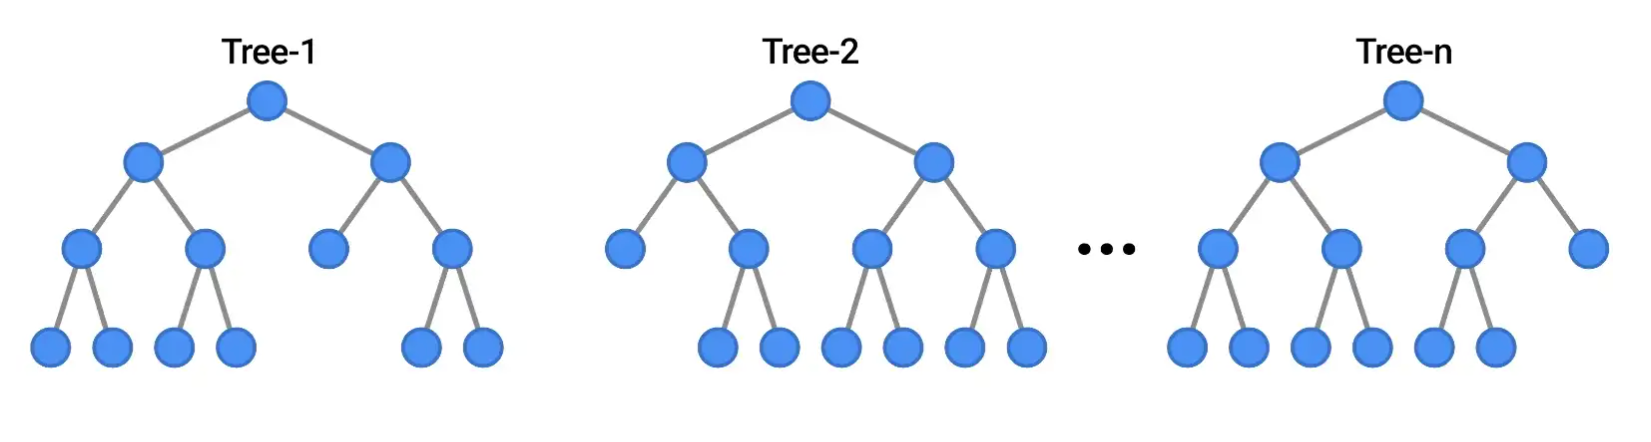
\includegraphics[width=0.8\textwidth]{../figures/Decision_tree.png}
    \caption{A simple ilustration of a Random Forest with n trees and a max depth of 3. \href{https://towardsdatascience.com/how-do-random-forests-decision-trees-decide-simply-explained-with-an-example-in-python-6737eb183604}{Refference} (Visited on 16. Dec 2022) }
    \label{fig:tree}
\end{figure}
A problem one may face when using a single decision tree is overfitting. This can be explained by how a tree can have so many nodes that every sample in the training set will be perfectly classified. This can be solved by introducing stopping criteria such as restricting the maximum depth referring to the maximum number of splits one branch is allowed to make. We can also introduce more trees trained on different data subsets, making a forest. This is done in a Random Forest, where each subset includes bootstrapped data from the original dataset. What is special about a Random Forest is how the branch splitting is done. Instead of using all $p$ predictors when performing each split, we randomly select $m \leq p$. This makes it possible for the trees to look very different from each other, because of the strongest predictor not always being among the $m$ randomly chosen predictors, leaving us with these predictors not always being in the upper branches. Therefore, we can get different predictions from each tree, which averaged will give the whole forest's final prediction. This way of averaging over many now uncorrelated trees makes a great reduction in variance compared to a single decision tree. We will implement the Random Forest by using TensorFlow. The code for this can be found on \href{https://github.com/Fslippe/FYS-STK4155/tree/main/project3}{GitHub}.
% subsection Implementation of methods (end)



\section{Results}
\label{sec:Results}

\subsection{Data correlation} % (fold)

% subsection Data correlation (end)
% subsection  (end)
To get a better understanding of the dataset we find the fraction of days with, and with no rain tomorrow for the different datasets as seen in table \ref{tab:frac}.
\begin{table}[H]
    \begin{small}
        \caption{Fraction of days with rain tomorrow and no rain tomorrow for different weather stations.}
        \label{tab:frac}
        \begin{center}
            \begin{tabular}{|l|l|l|}
                \hline
                \textbf{Weather station(s)} & \textbf{Days with rain tomorrow} & \textbf{Days with no rain tomorrow} \\
                \hline
                Cobar                       & 11.8\%                           & 88.2\%                              \\
                \hline
                Coffs Harbour               & 31.2\%                           & 68.8\%                              \\
                \hline
                Darwin                      & 25.8\%                           & 74.2\%                              \\
                \hline
                All stations                & 22.0\%                           & 78.0\%                              \\
                \hline
            \end{tabular}
        \end{center}
    \end{small}
\end{table}
We see different fractions of rain tomorrow for the three different weather station with Cobar only having rain 11.8\% of the days. We notice that the average fraction of rain days for all weather stations is at 22\% with Darwin being close to this average at 25.8\%. Coffs Harbour show similar to Cobar a large deviation from the mean, but with a higher fraction than the average arriving at 31.2\%.

We continue gaining more insight of the dataset by plotting the correlation matrix as seen in figure \ref{fig:corr}
\begin{figure}[H]
    \centering
    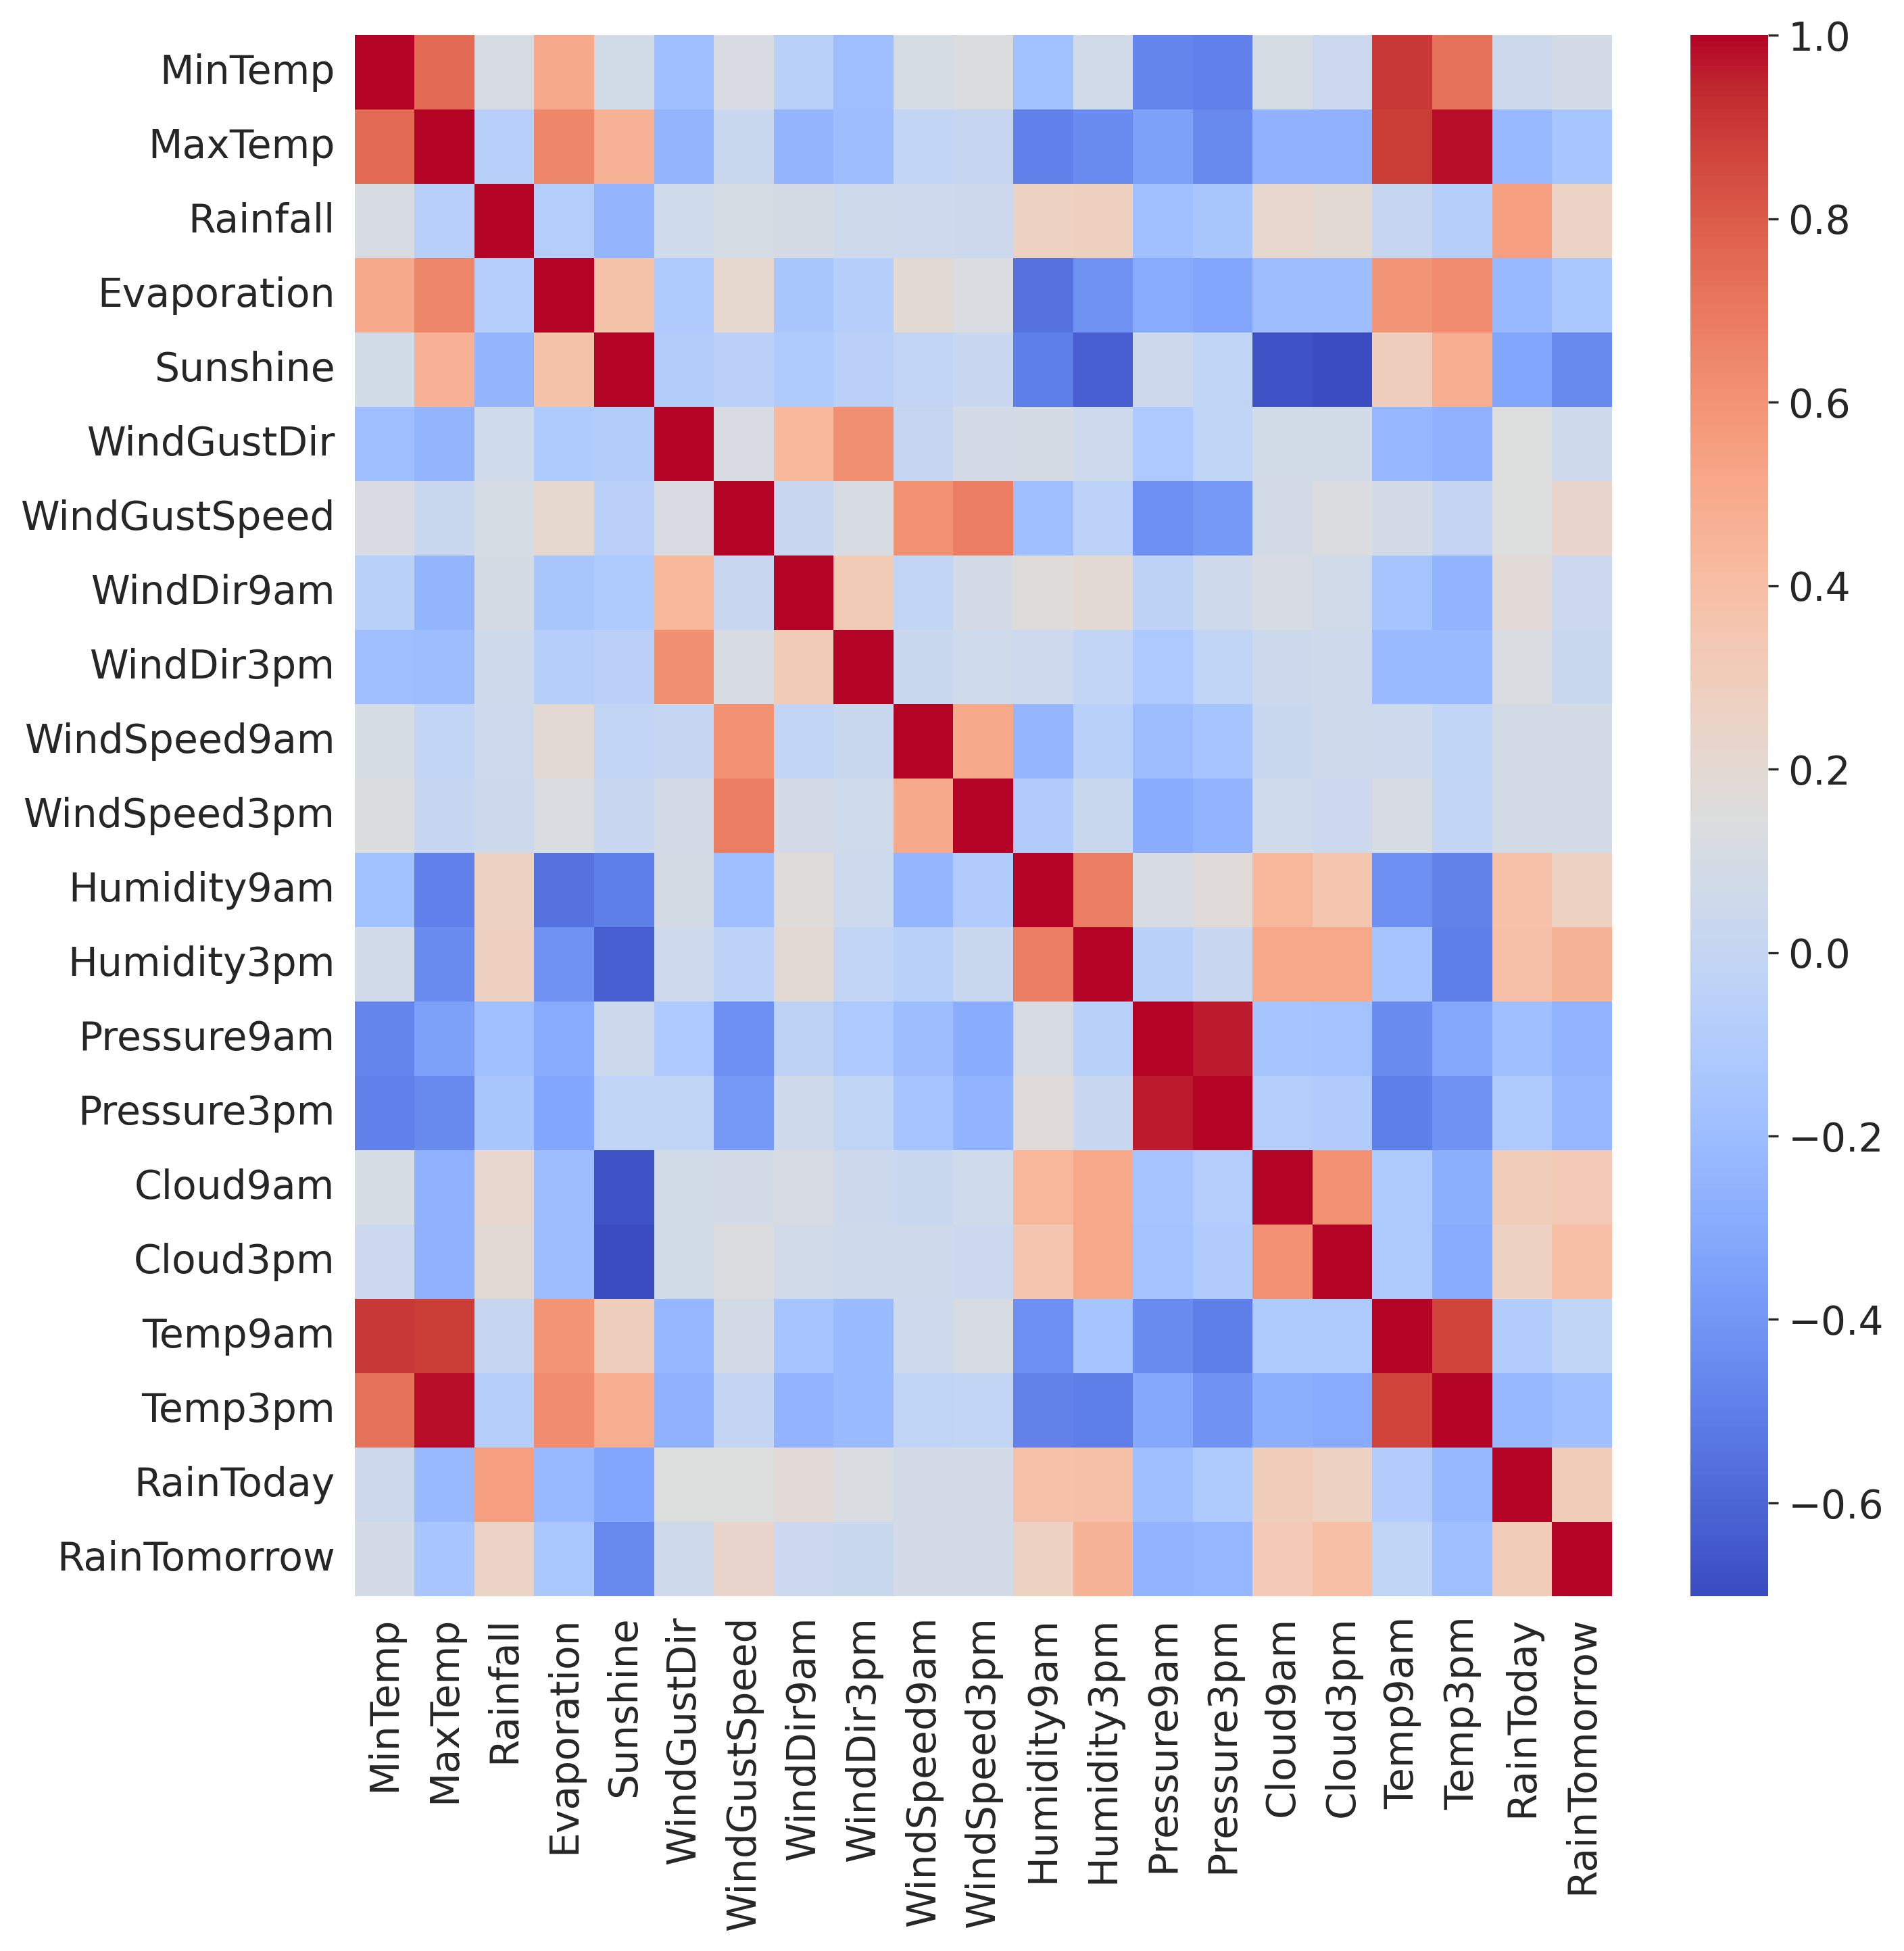
\includegraphics[width=0.8\textwidth]{../figures/correlation_heatmap_full.png}
    \caption{Correlation between the different features of the dataset.}
    \label{fig:corr}
\end{figure}

In our case of mainly looking at how today's weather influences tomorrow's weather is the bottom row or the rightmost column in figure \ref{fig:corr} what interests us. We see that the different features influences the feature \textit{RainTomorrow} to different degrees. Number of sunshine hours is the feature with the most negative correlation while the humidity at 3pm is the feature with the most positive correlation.

In figure \ref{fig:features} we see how different weather stations deviate from the mean for the two most \textit{RainTomorrow} correlated features. We see sunshine hours in \ref{fig:sunshine} and humidity in \ref{fig:humidity}. In the sunshine plot we notice the stations Cobar, Coffs Harbour and Darwin having more sunshine than the mean with Coffs Harbour deviating the most with close to 2 extra sunshine hours more than the mean each day. In the humidity plot we see Cobar having close to the mean humidity and that both Coffs Harbour and Darwin deviate from the mean with close to -25 and -15 percent respectively.
\begin{figure}[H]
    \begin{subfigure}{\textwidth}
        \centering
        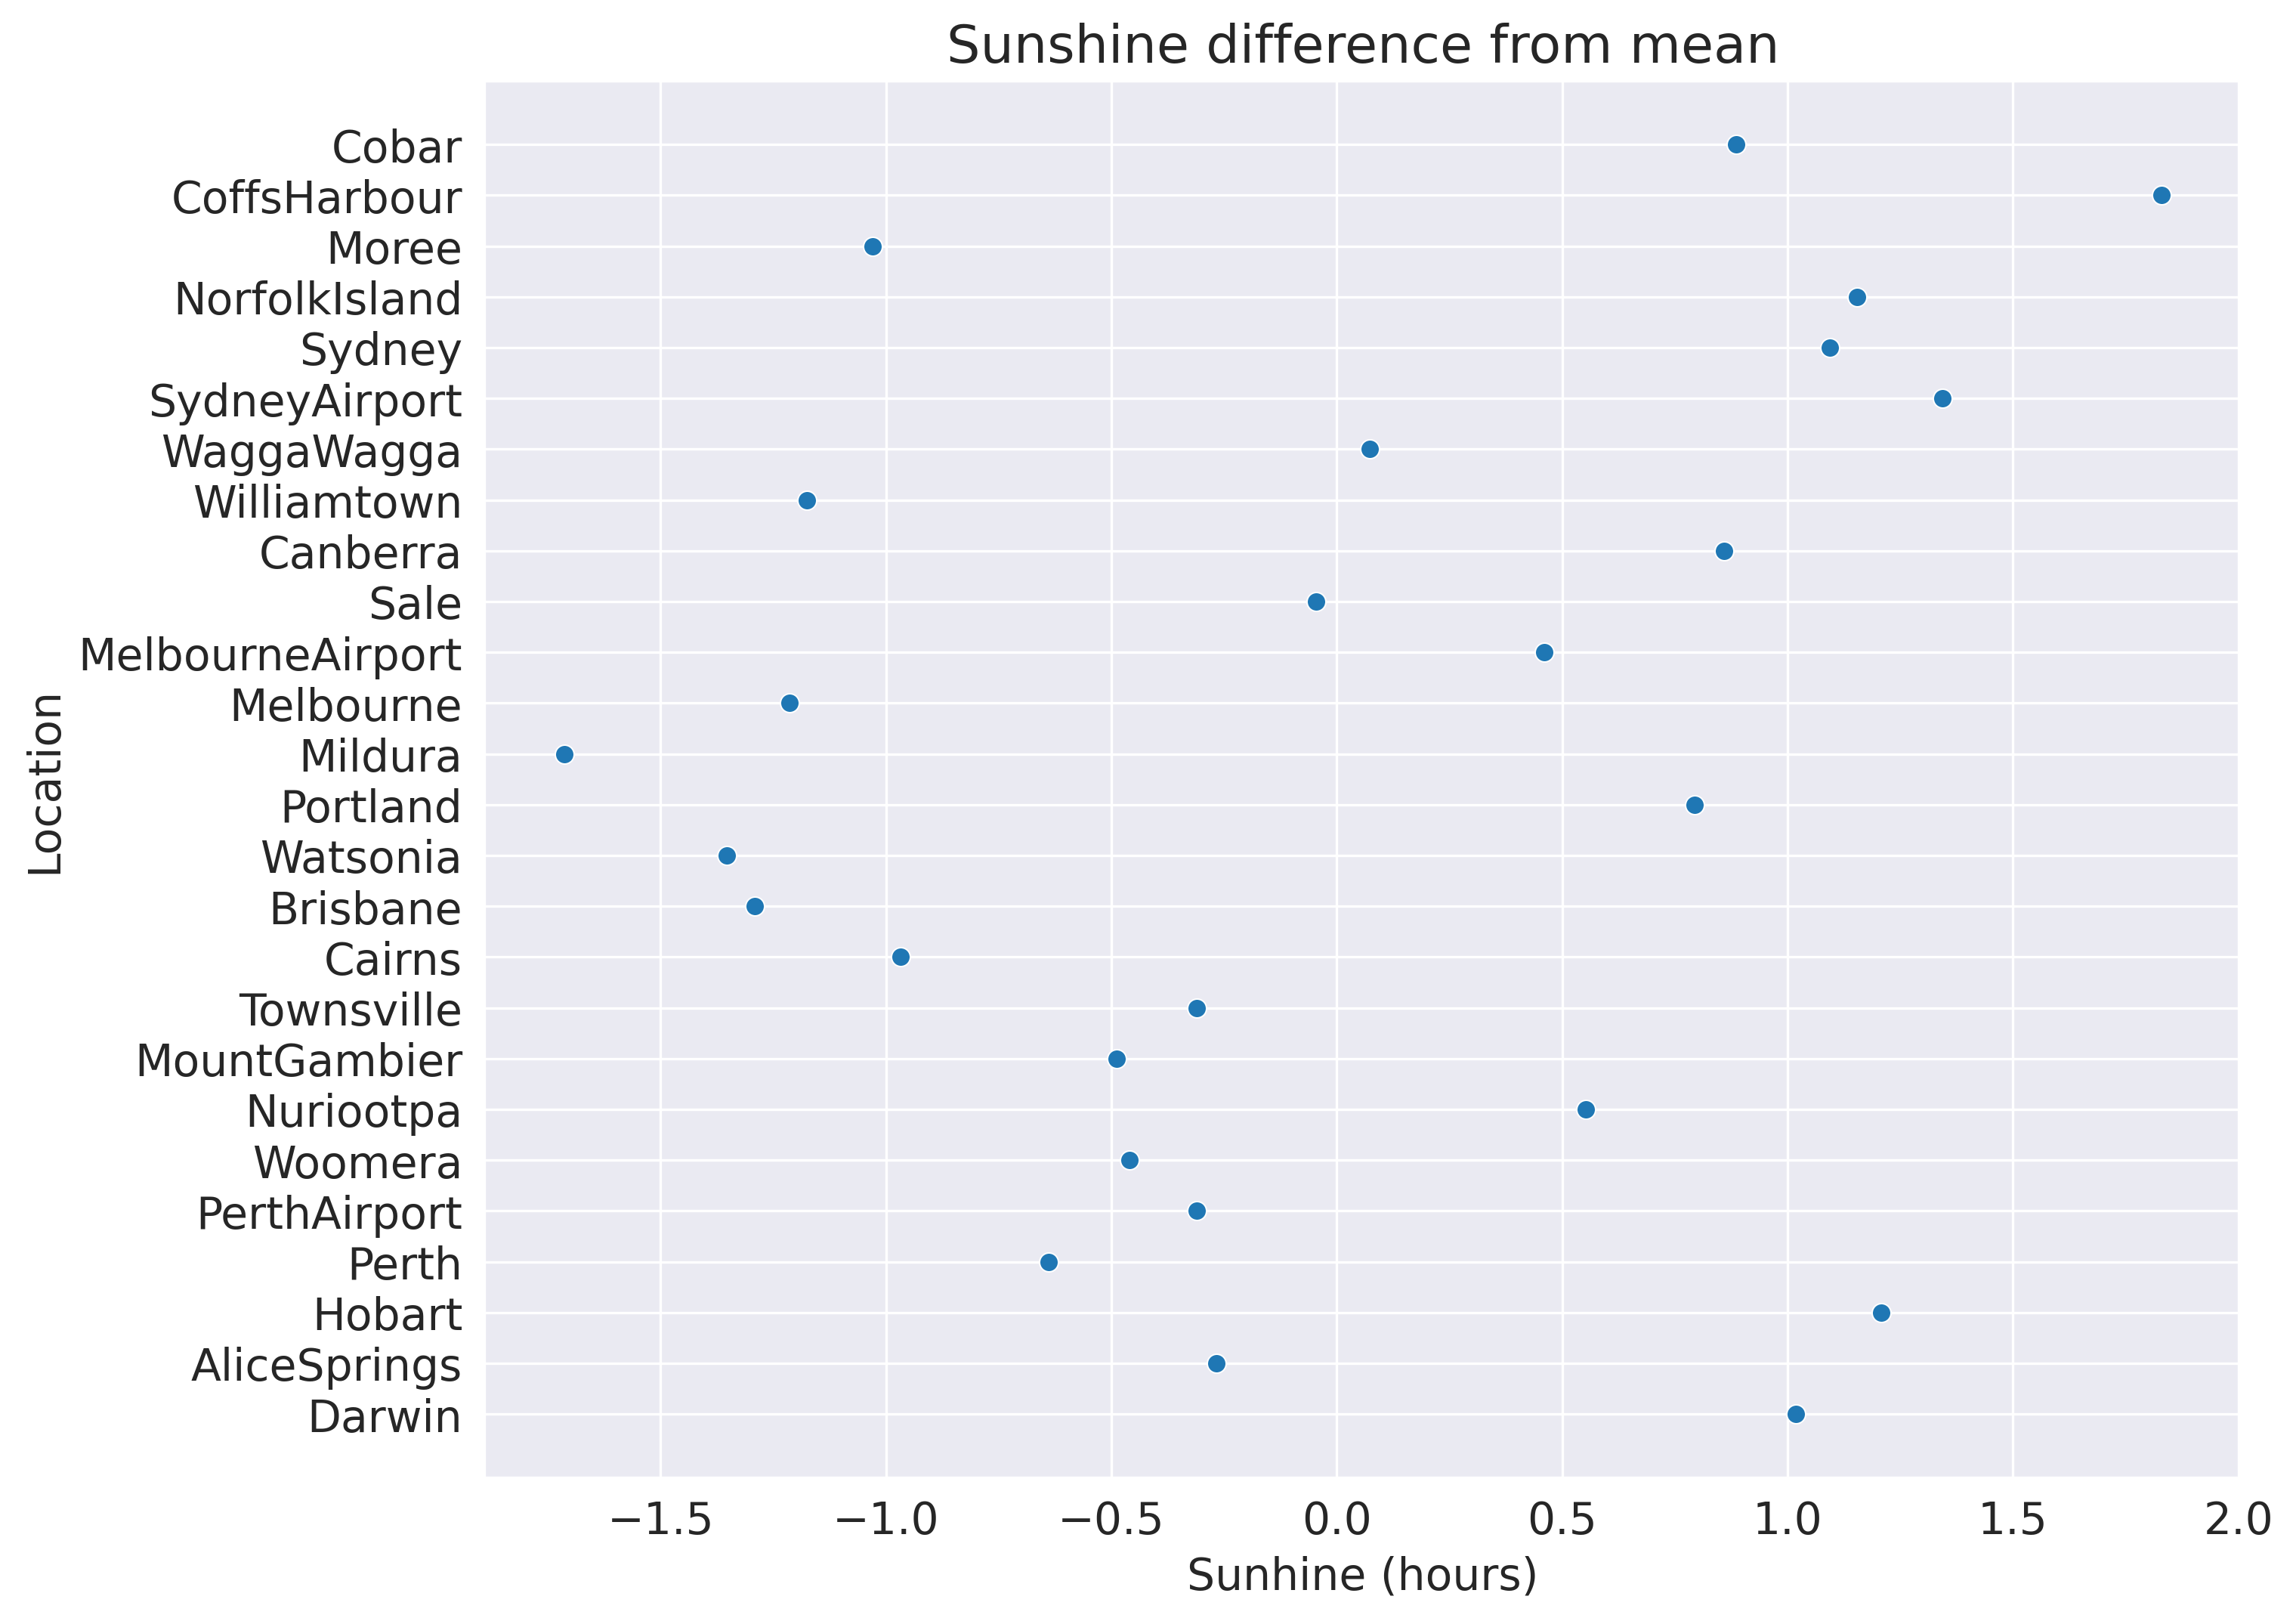
\includegraphics[width=.8\textwidth]{../figures/Sunshine.png}
        \caption{Deviation in daily sunshine hours from the mean.}
        \label{fig:sunshine}
    \end{subfigure}
    \begin{subfigure}{\textwidth}
        \centering
        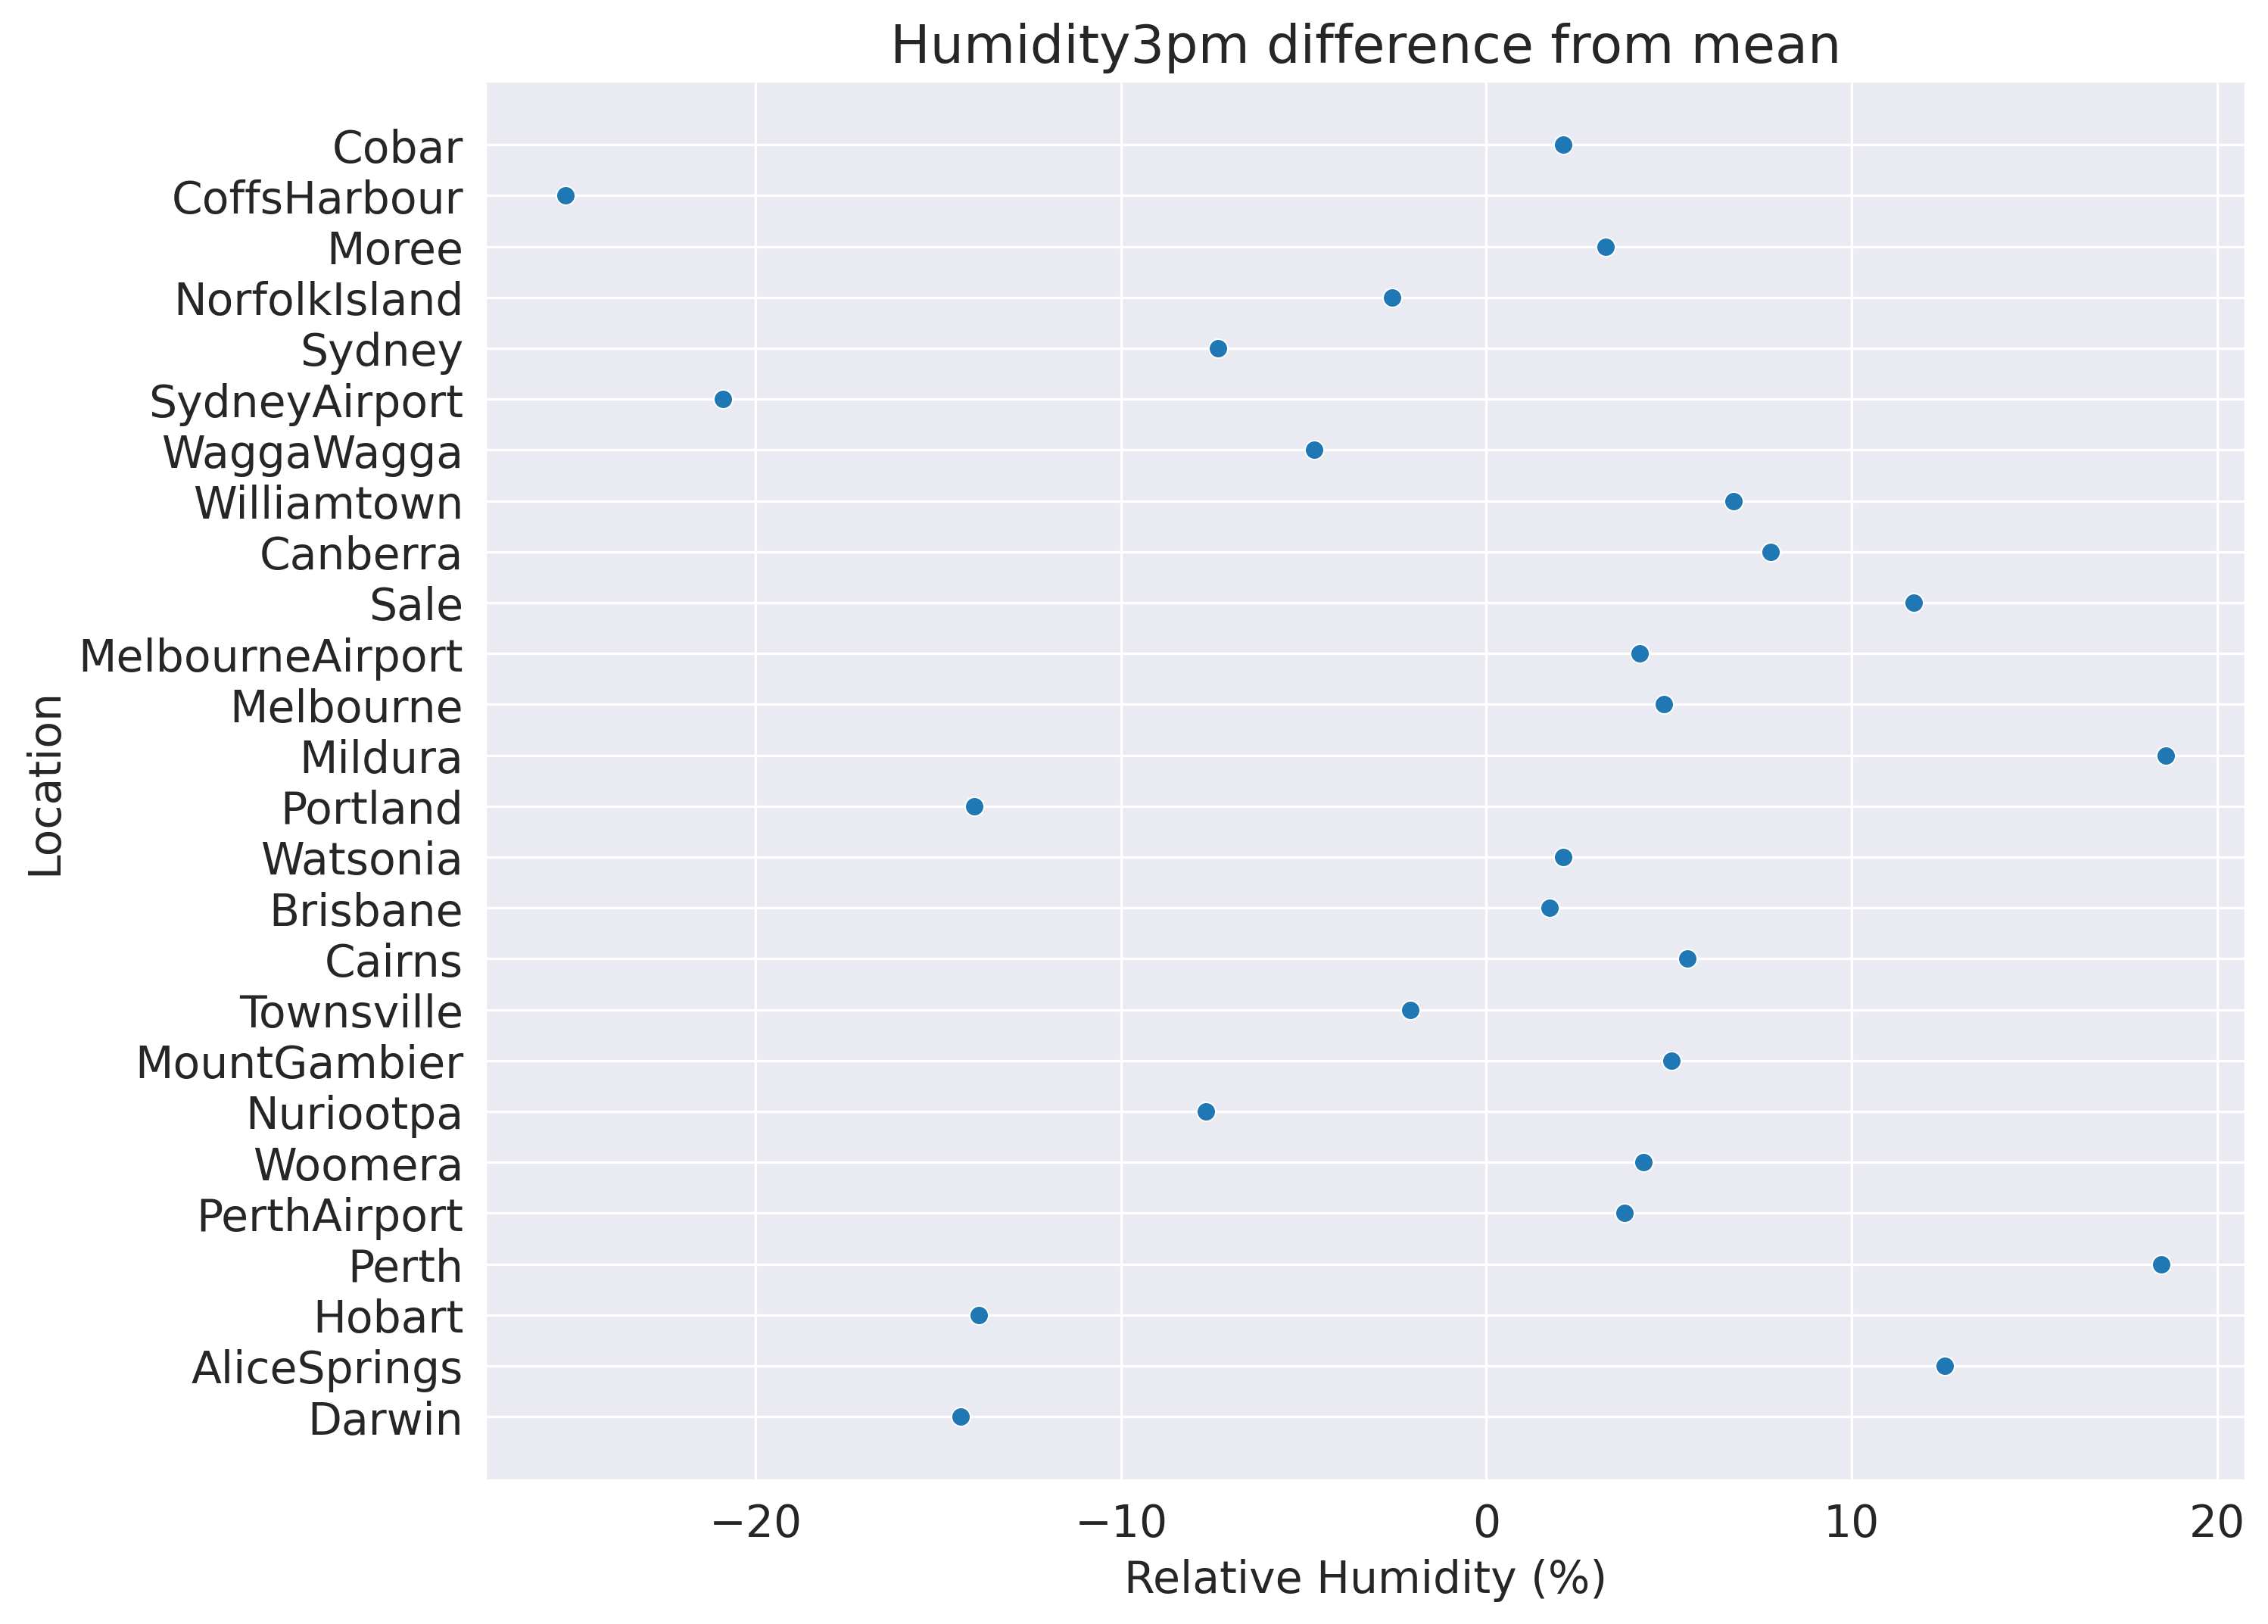
\includegraphics[width=.8\textwidth]{../figures/Relative_humidity3pm.png}
        \caption{Deviation in relative humidity at 3pm from the mean.}
        \label{fig:humidity}
    \end{subfigure}
    \caption{Deviations from the mean for the different weather stations. We see deviation in daily sunshine hours in \ref{fig:sunshine} and deviations in relative humidity at 3pm in \ref{fig:humidity}.}
    \label{fig:features}
\end{figure}
\newpage


\subsection{Predictions using a single station}
Our first tests include a layer-neurons grid search for the Neural Network, a learning rate L2-norm grid search for logistic regression, and a trees-depth grid search for Random Forest. For the Neural Network and the logistic regression we perform the grid search using both ADAM and Stochastic Gradient Decent as optimizers for the gradient decent as seen in figure \ref{fig:cobar_grid} and \ref{fig:cobar_grid_logreg}. Similarly, we see a Random Forest grid search in figure \ref{fig:cobar_grid_rf}.
\begin{figure}[H]
    \begin{subfigure}{.5\textwidth}
        \centering
        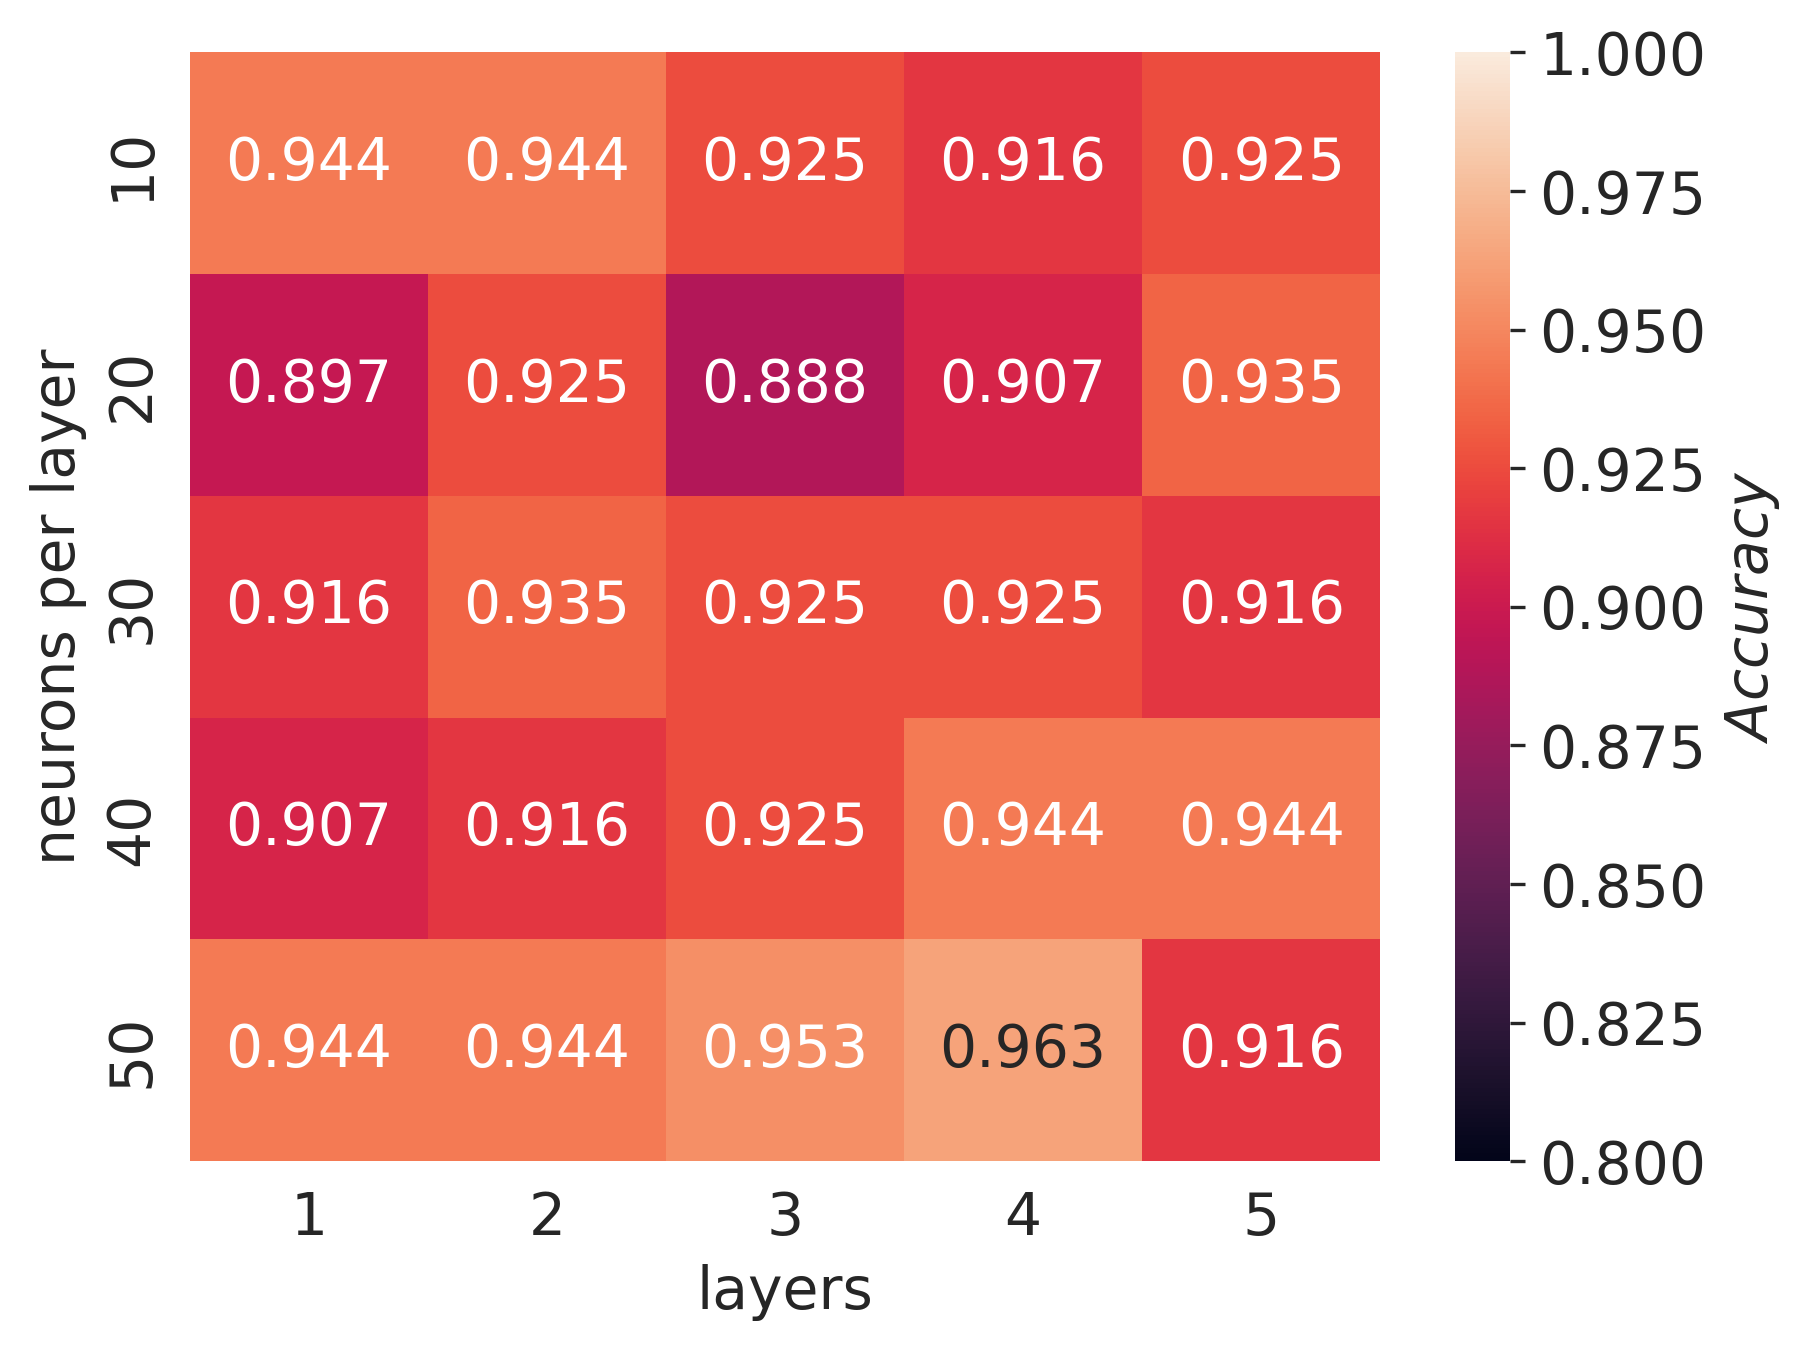
\includegraphics[width=\textwidth]{../figures/NN_grid_SGD_bootstrap_cobar.png}
        \caption{SGD}
        \label{fig:}
    \end{subfigure}
    \begin{subfigure}{.5\textwidth}
        \centering
        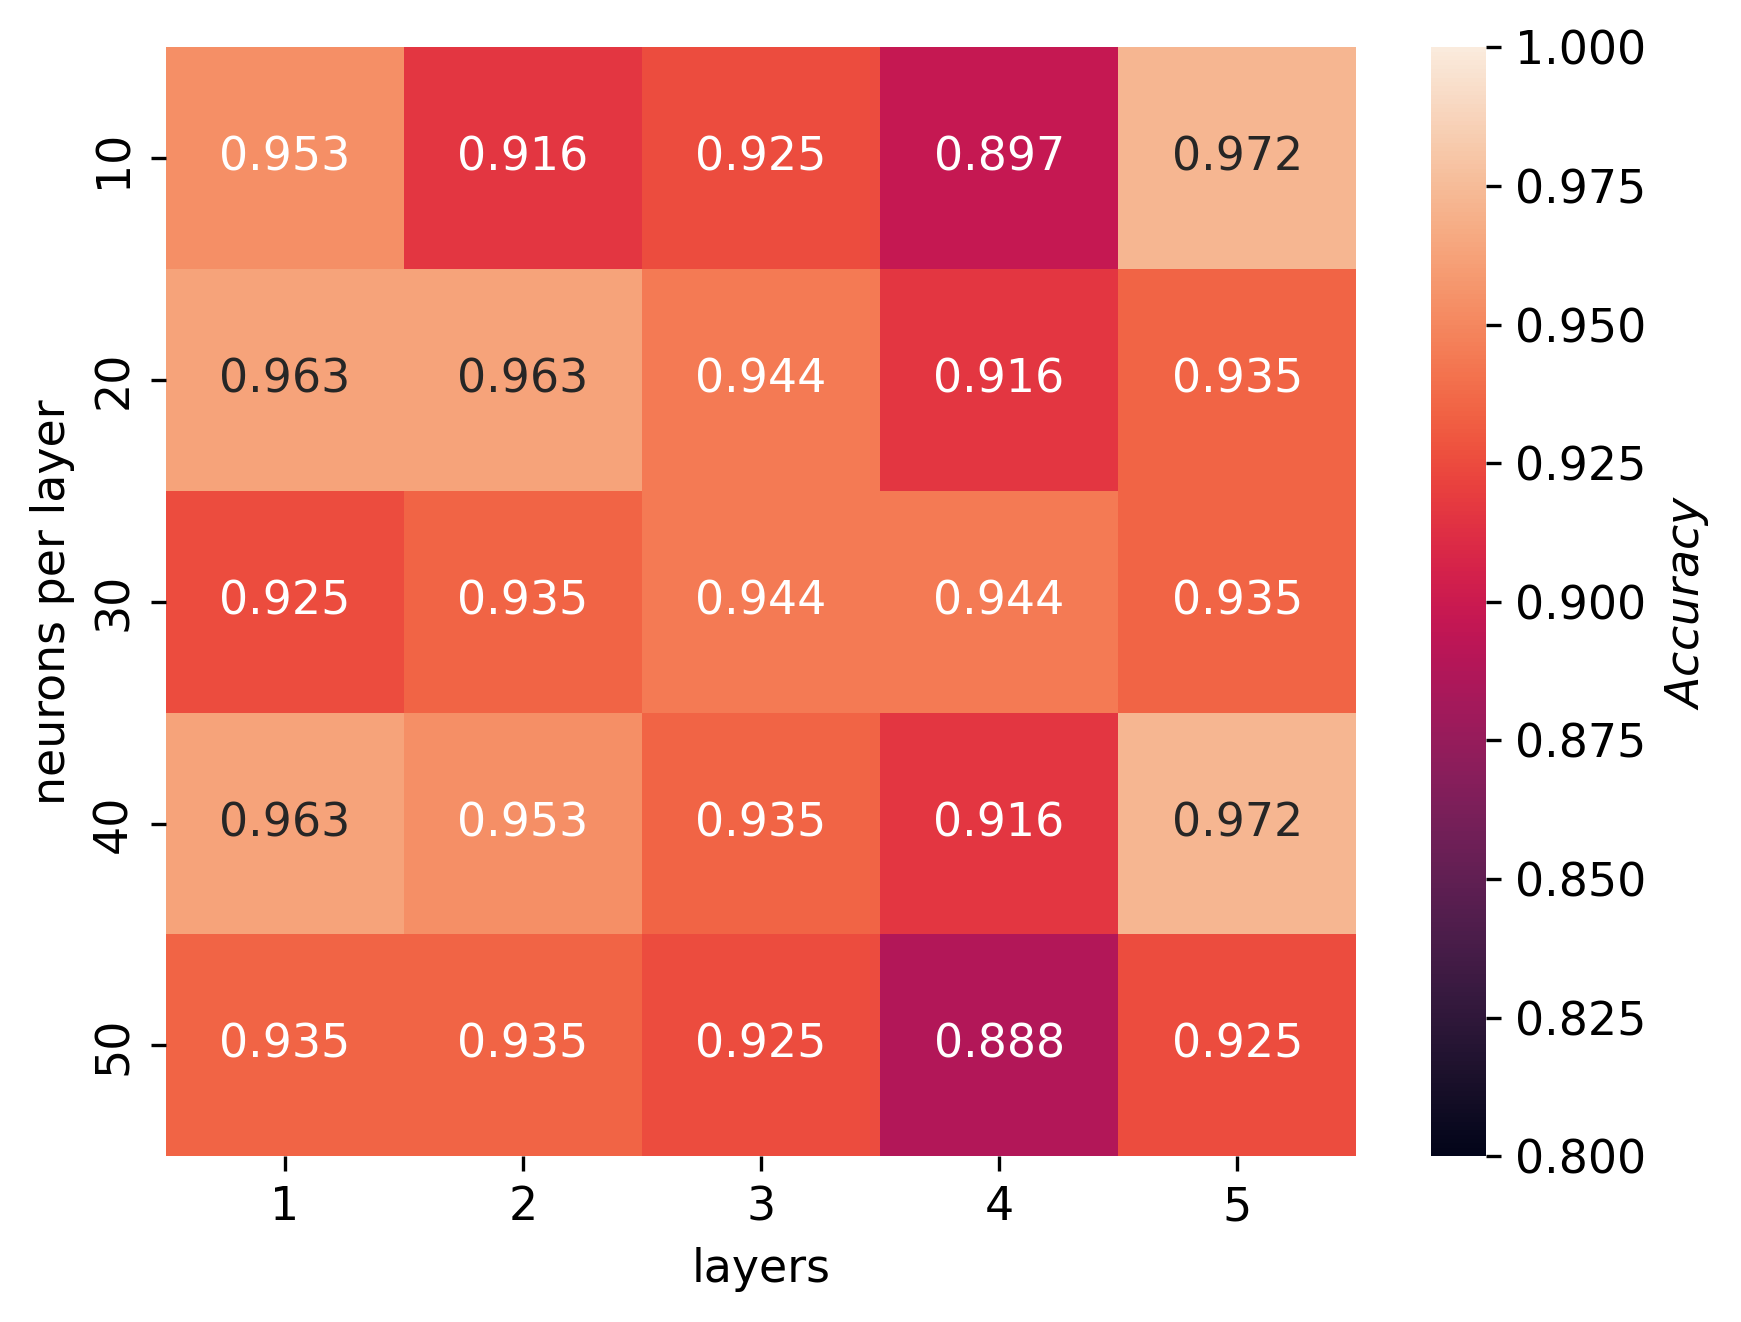
\includegraphics[width=\textwidth]{../figures/NN_grid_ADAM_bootstrap_cobar.png}
        \caption{ADAM}
        \label{fig:}
    \end{subfigure}
    \caption{Grid search using 10 bootstrap iterations for different number of neurons and hidden layers in a TensorFlow sequential Neural Network. ReLU has been used as activation for the hidden layers, and sigmoid for the output layer. Binary crossentropy has been used as loss function. A batch size of 32 together with 100 epochs has been used. All other parameters have been automatically chosen by TensorFlow.}
    \label{fig:cobar_grid}
\end{figure}
\begin{figure}[H]
    \begin{subfigure}{.5\textwidth}
        \centering
        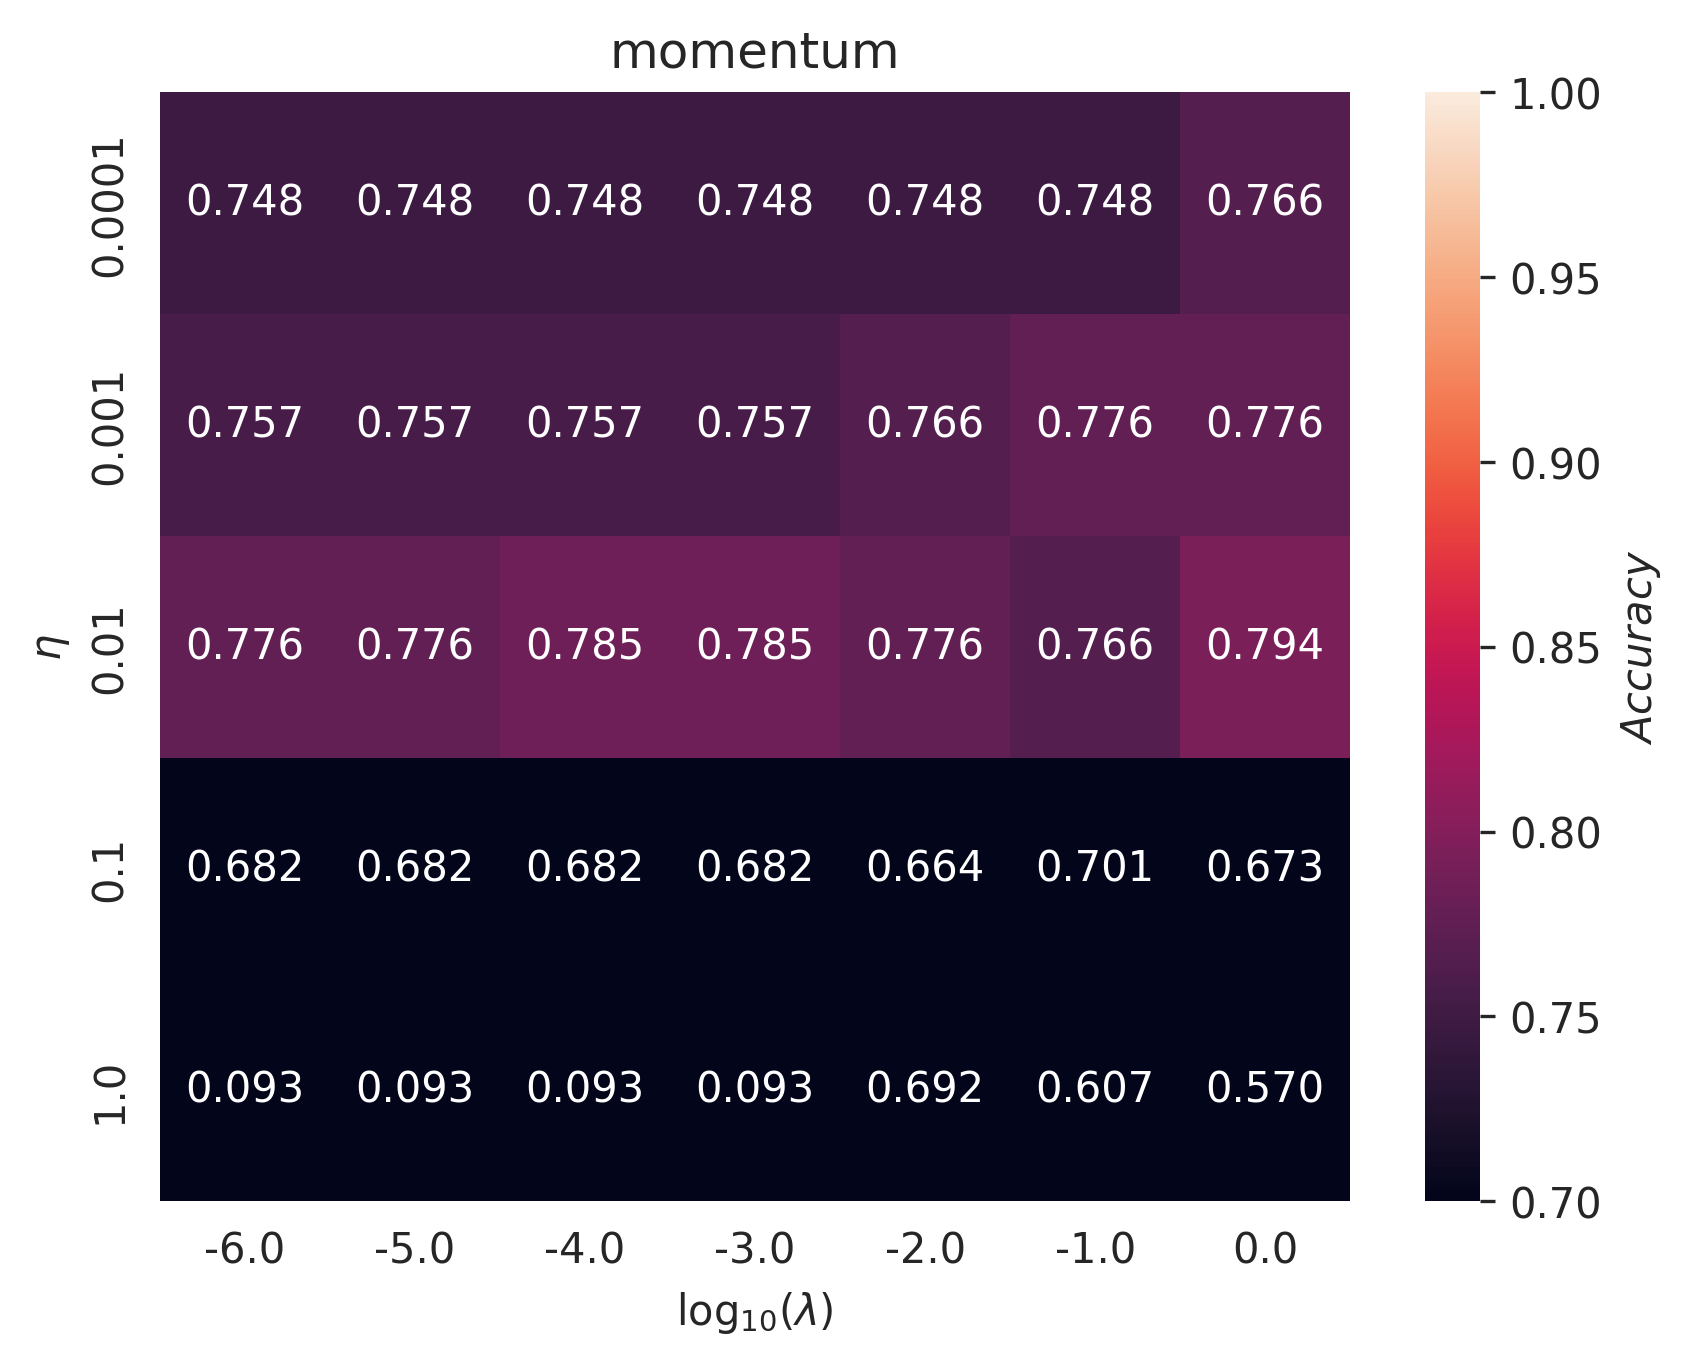
\includegraphics[width=\textwidth]{../figures/logreg_momentum_Cobar.png}
        \caption{SGD}
        \label{fig:}
    \end{subfigure}
    \begin{subfigure}{.5\textwidth}
        \centering
        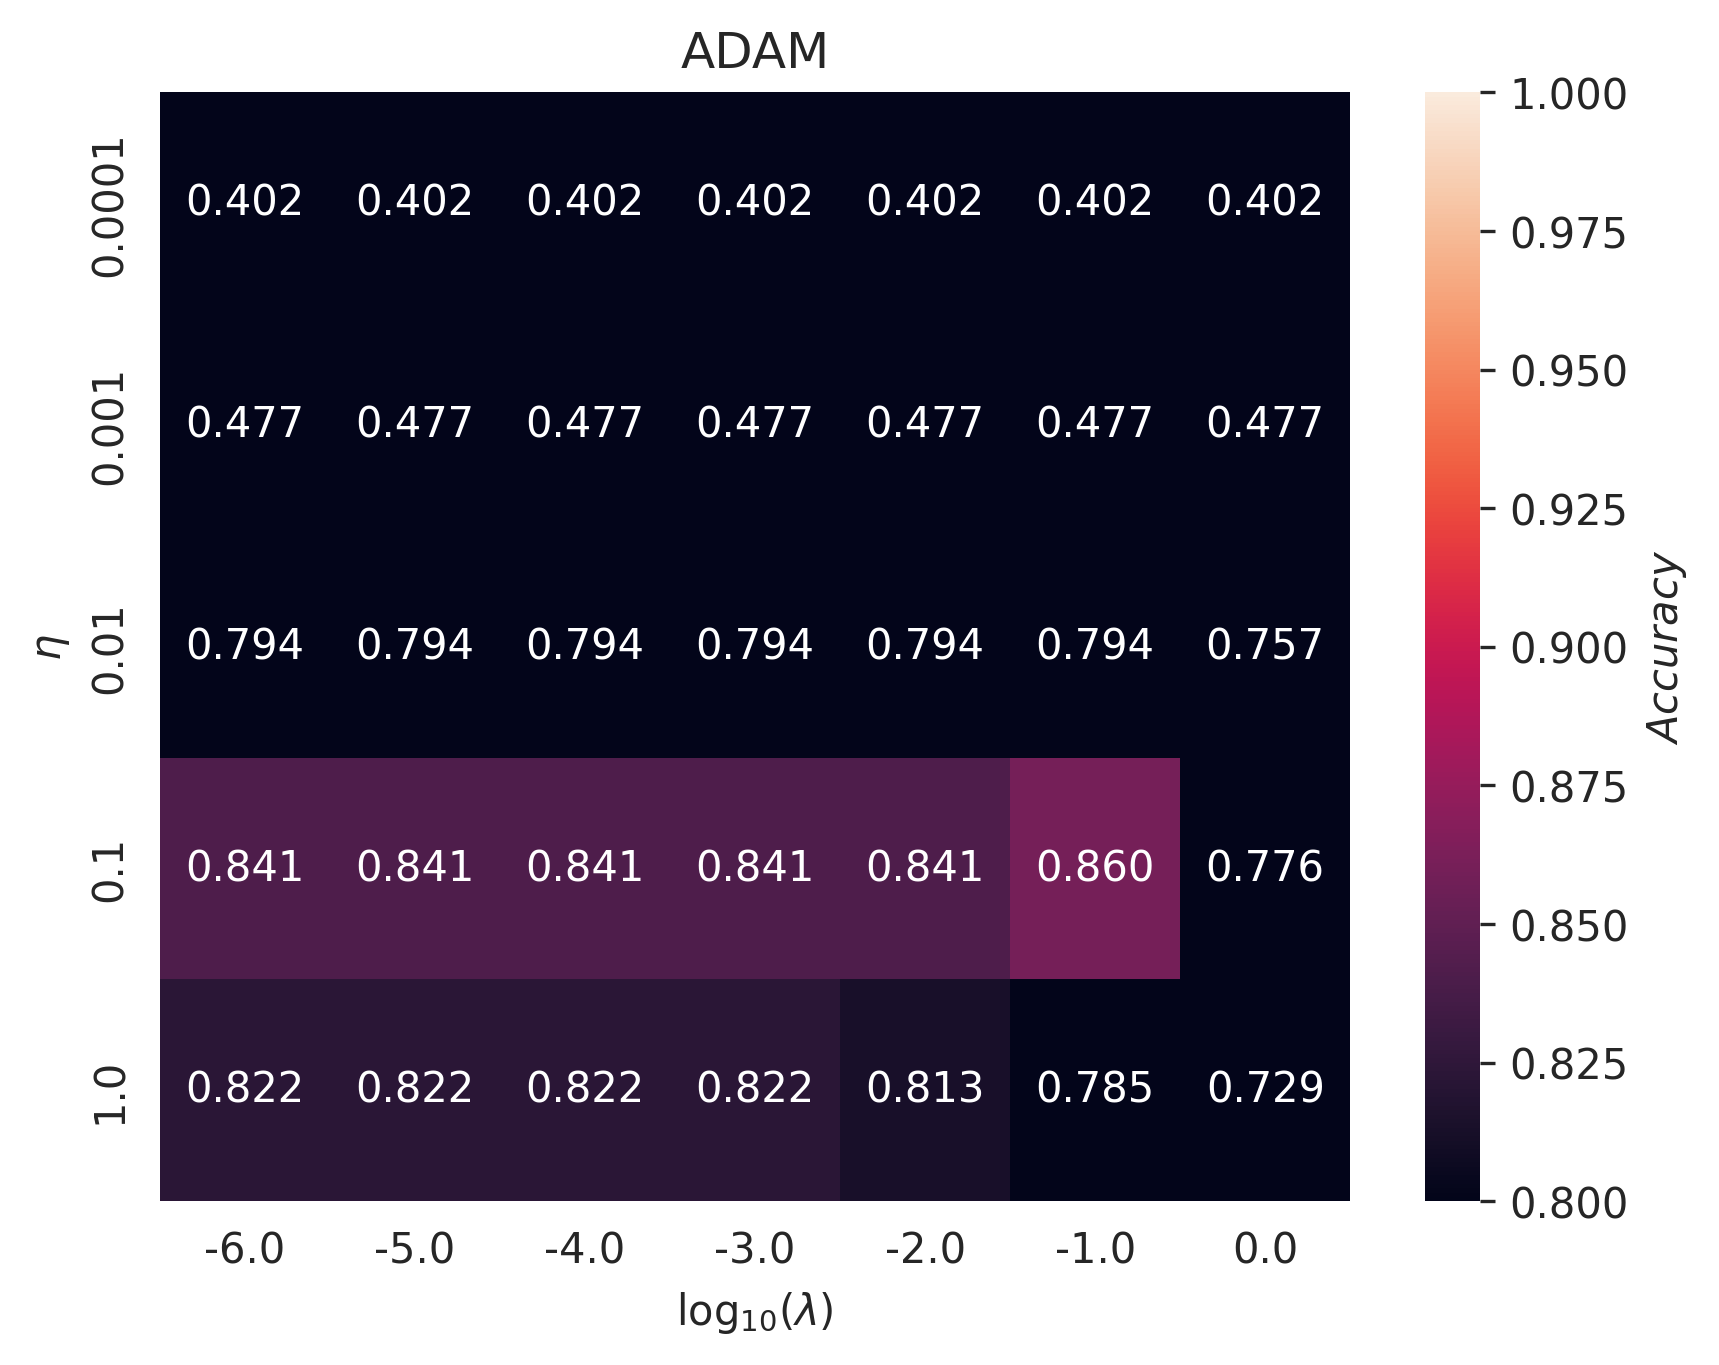
\includegraphics[width=\textwidth]{../figures/logreg_ADAM_Cobar.png}
        \caption{ADAM}
        \label{fig:}
    \end{subfigure}
    \caption{Grid search using 10 bootstrap iterations for different learning rates ($\eta$) and L-2 norm ($\lambda$) for logistic regression. Momentum of 0.3, a batch size of 32 together with 100 epochs have been used.}
    \label{fig:cobar_grid_logreg}
\end{figure}
\begin{figure}[H]
    \centering
    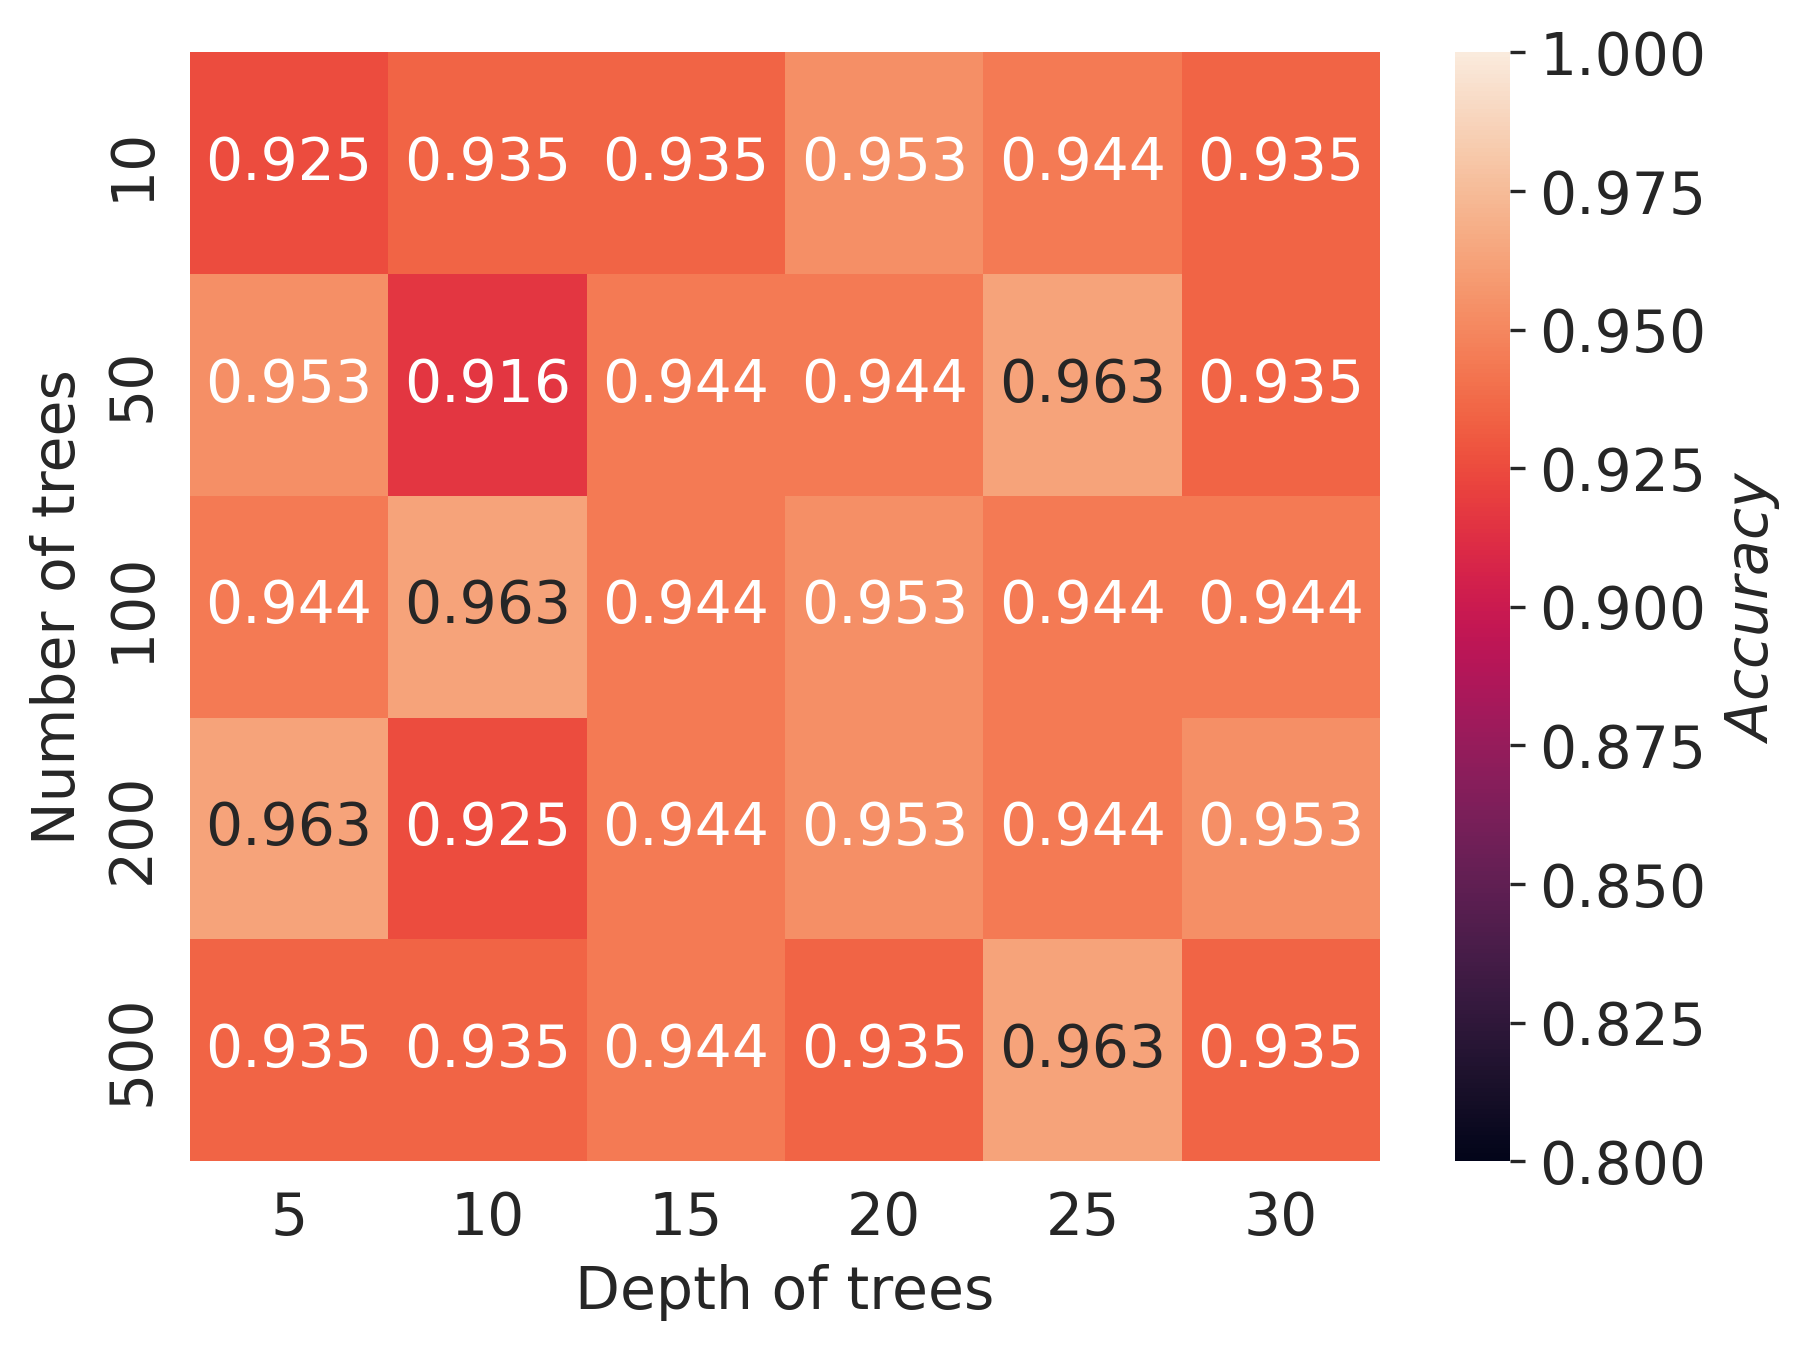
\includegraphics[width=0.5\textwidth]{../figures/RF_grid_bootstrap_cobar.png}
    \caption{Grid search using 10 bootstrap iterations for different number and depth of trees for a TensorFlow Random Forest model. All other parameters are chosen automatically by \href{https://www.tensorflow.org/decision_forests/api_docs/python/tfdf/keras/RandomForestModel}{TensorFlow}.}
    \label{fig:cobar_grid_rf}
\end{figure}

We see that the performance in both figure \ref{fig:cobar_grid}, \ref{fig:cobar_grid_logreg} and \ref{fig:cobar_grid_rf} vary depending on the parameters tested. The Neural Network performs slightly better than the Random Forest, and they both perform a lot better than the logistic regression. When comparing the results to table \ref{tab:frac} we see that the logistic regression performes worse than if it would predict no rain every day. In total, the grid search shows that only the neural network and the Random Forest perform well enough, and ready for further analysis.  The optimal parameters for the two models can be found below in table \ref{tab:grid_NN} and \ref{tab:grid_RF}.
\subsection{Predictions using all data}
We look at a dataset containing all weather stations and perform a grid search for the Random Forest and neural network as shown in figure \ref{fig:grid_full}.
\begin{figure}[H]
    \begin{subfigure}{.5\textwidth}
        \centering
        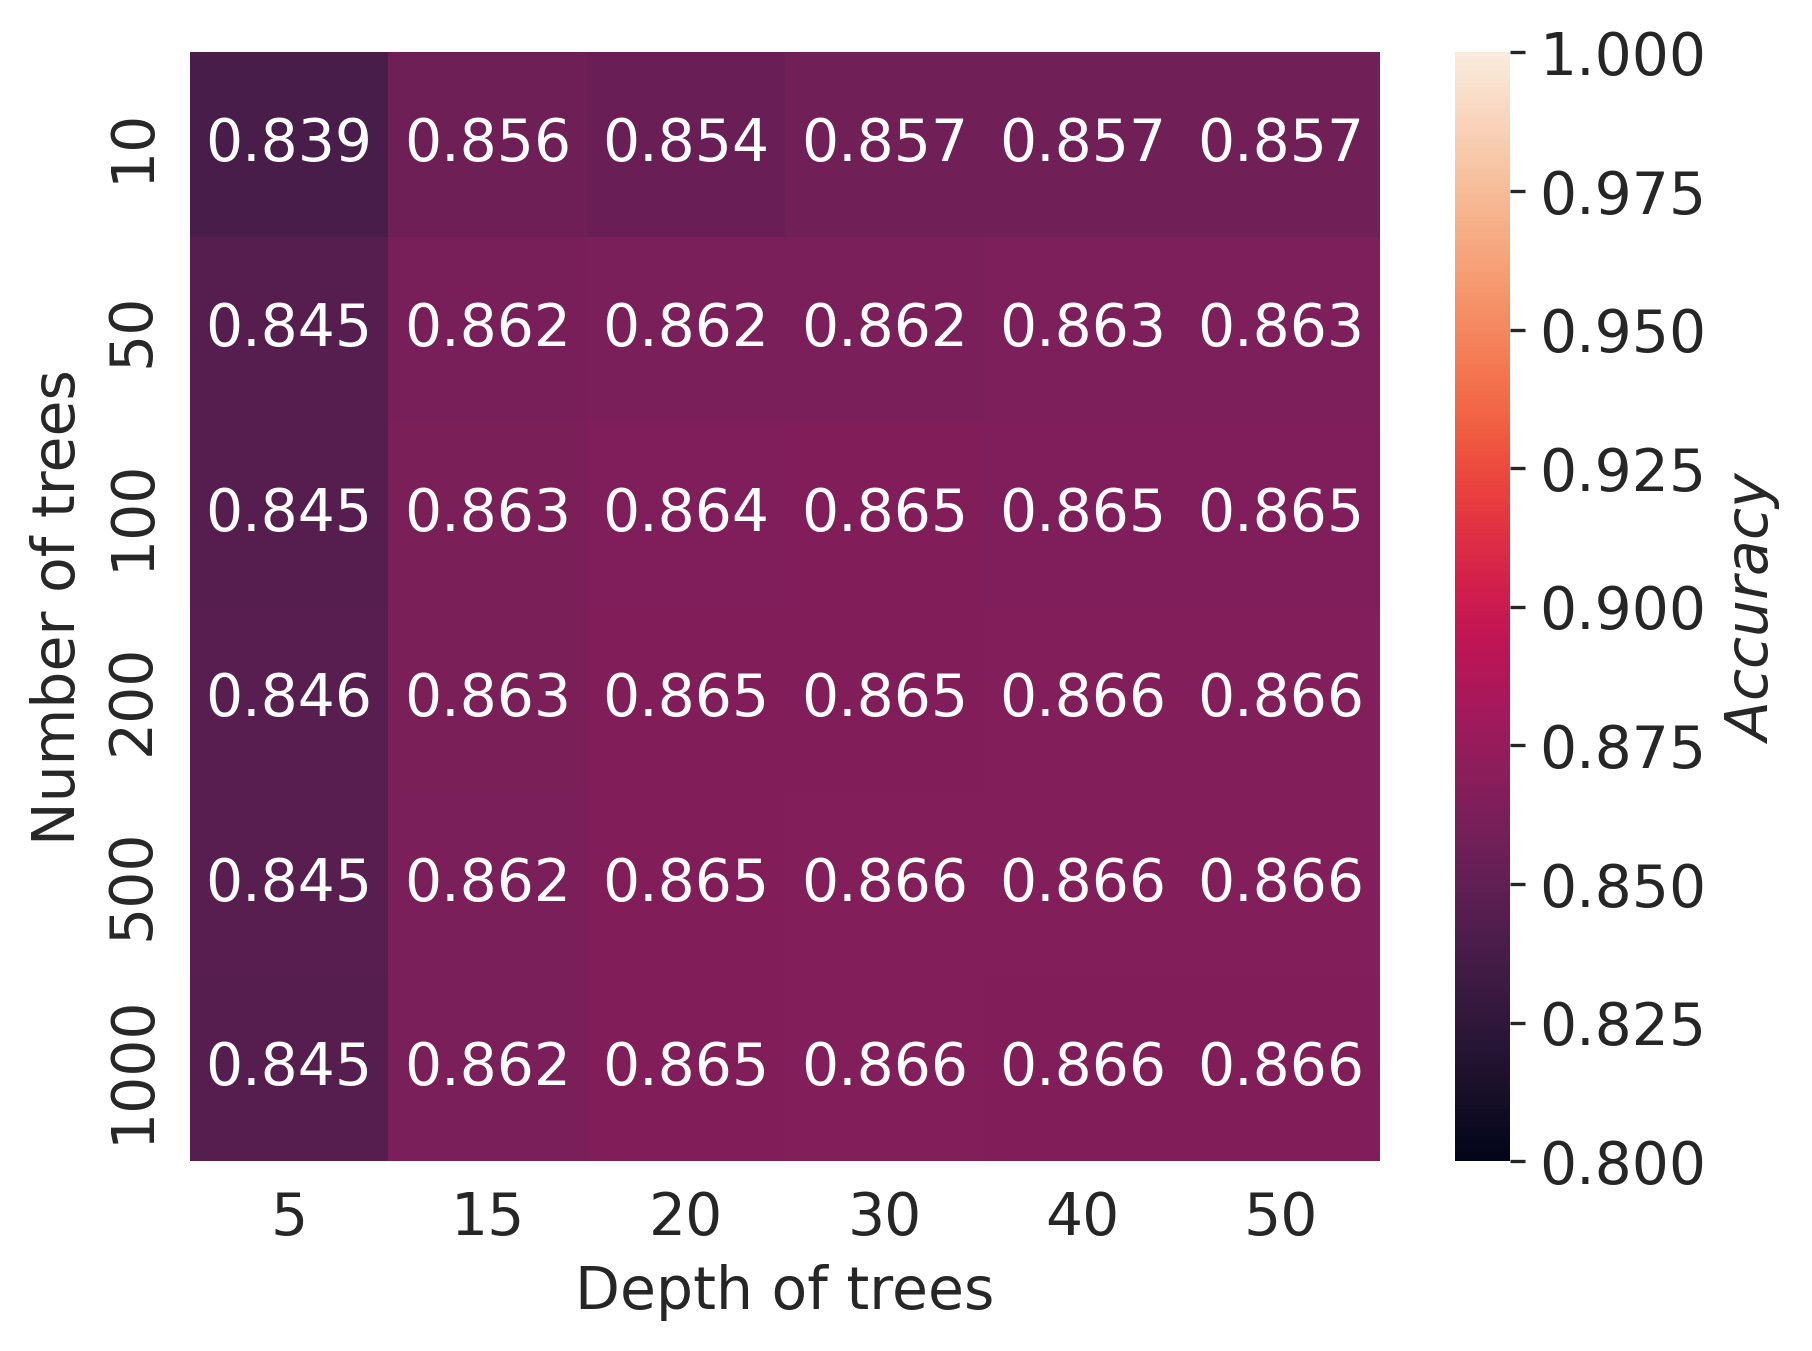
\includegraphics[width=\textwidth]{../figures/RF_grid_all.png}
        \caption{Random Forest}
        \label{fig:rf_full}
    \end{subfigure}
    \begin{subfigure}{.5\textwidth}
        \centering
        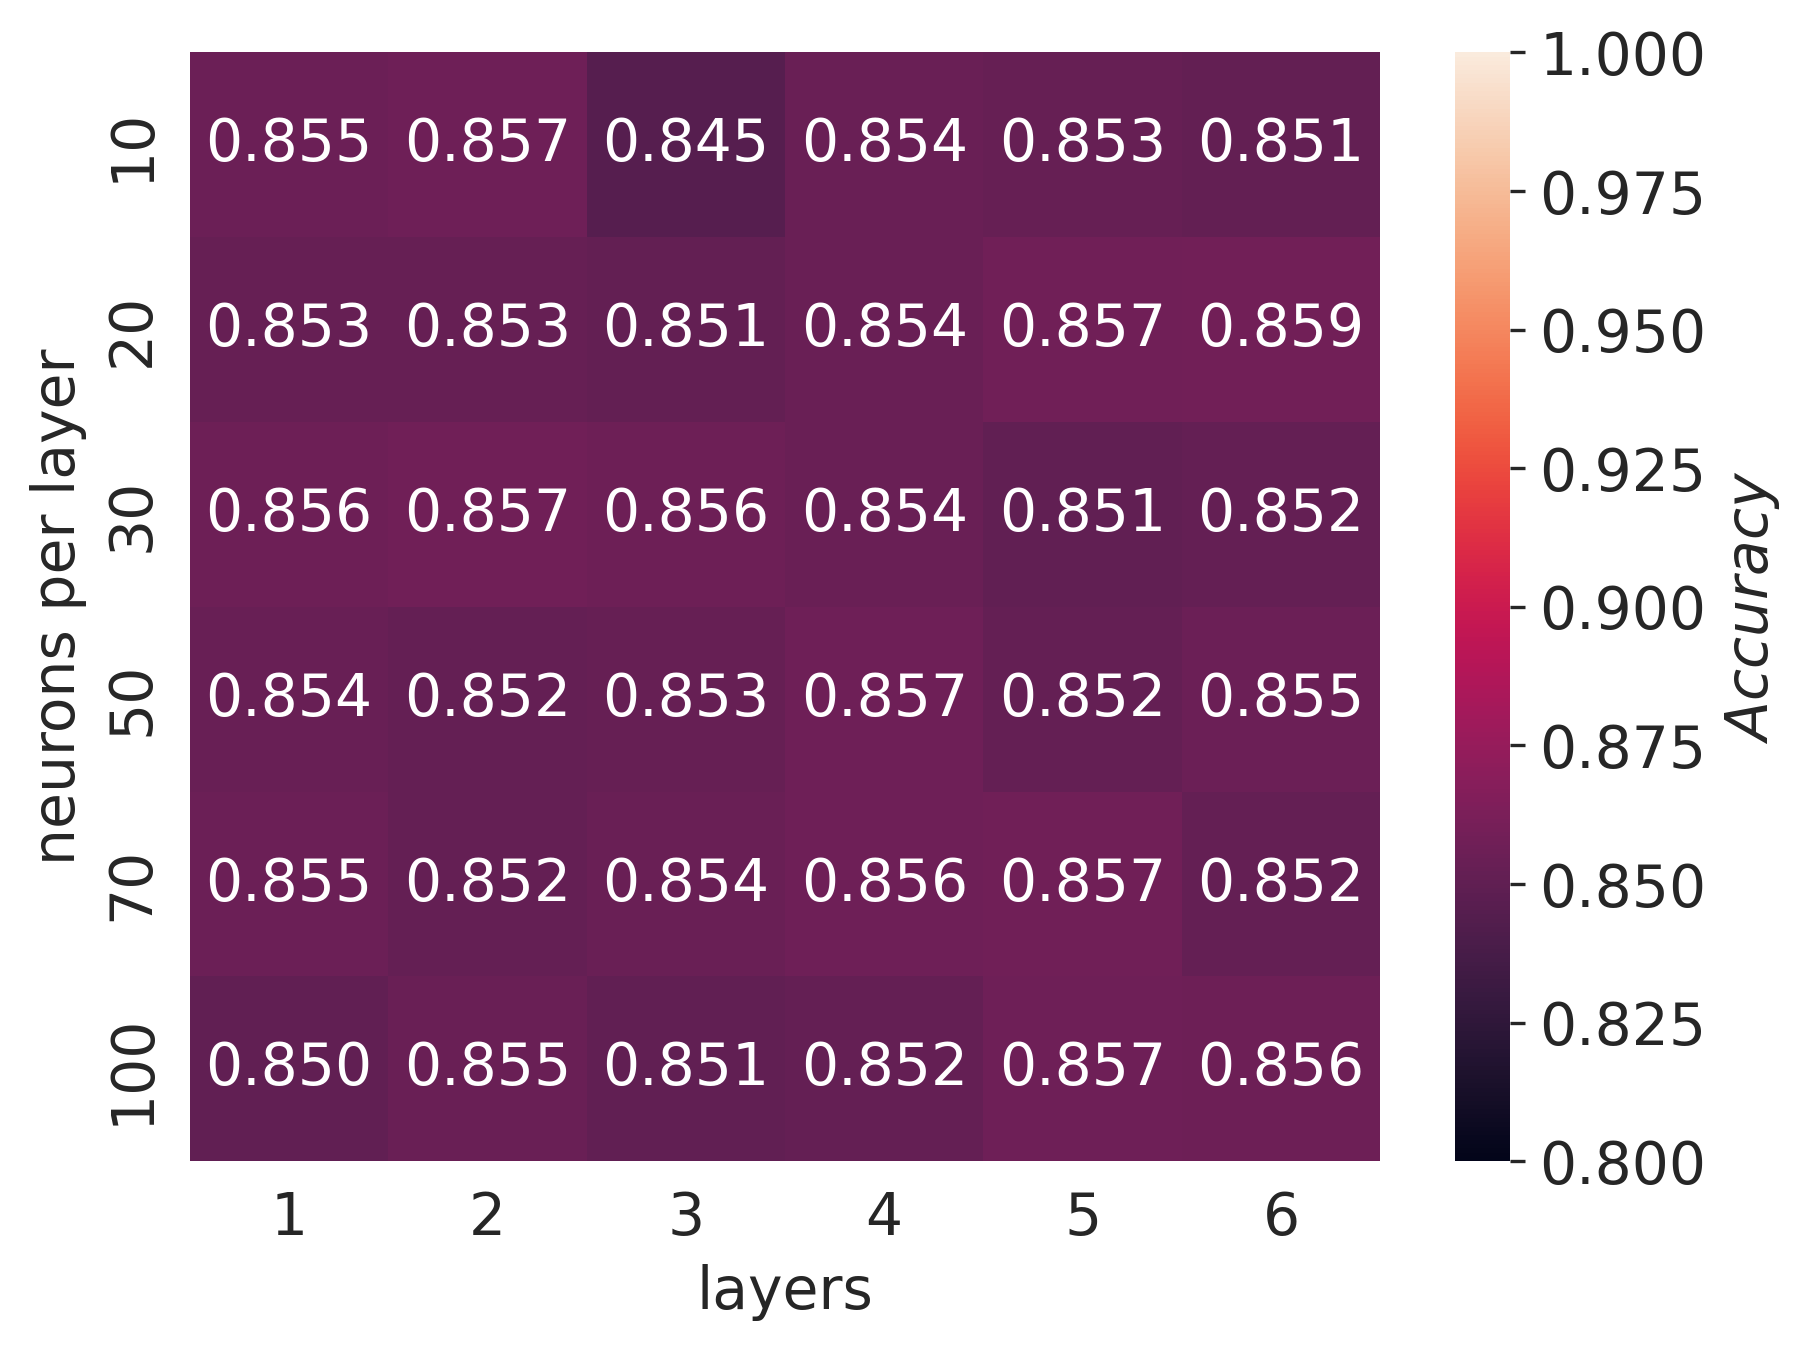
\includegraphics[width=\textwidth]{../figures/NN_grid_ADAM_all.png}
        \caption{Neural Network with ADAM}
        \label{fig:NN_full}
    \end{subfigure}
    \caption{Grid search using 10 bootstrap iterations for a Neural Network and a Random Forest. For the Neural Network, ReLU has been used as activation for the hidden layers, and sigmoid for the output layer. Binary crossentropy has been used as loss function. A batch size of 320 together with 100 epochs has been used. All other parameters for both the Neural Network and the Random Forest have been automatically chosen by TensorFlow \cite{tf}\cite{tfrf}.}
    \label{fig:grid_full}
\end{figure}

We see in \ref{fig:rf_full} that more trees and a larger depth generally equals a more accurate model. For the Neural Network wee see more variation and not a clear tendency with more neurons and layers equalling a more accurate model. The parameters used, and the highest accuracy found is shown in table \ref{tab:grid_RF}.

For our final analysis we use the optimal Neural Network and Random Forest models trained on all data to evaluate their predictions on specific weather stations. This can be seen for Cobar, Coffs Harbour and Darwin in table \ref{tab:grid_RF} for Random Forest, and in table \ref{tab:grid_NN} for the Neural Network.

\begin{table}[H]
    \caption{Accuracy on different datasets as train and test data using a Neural Network. 100 epochs has been used for both Cobar and full data. Batch size of 32 has been used for Cobar, and a batch size of 320 has been used for the full data as training dataset.  The optimal parameters used have been found using grid search in figure \ref{fig:cobar_grid} for Cobar, and in figure \ref{fig:NN_full} for full data as training data. Other parameters have been automatically chosen by TensorFlow \cite{tf}}
    \label{tab:grid_NN}
    \centering
    \begin{tabular}{|l|l|l|l|l|}
        \hline
        \textbf{Train Data}      & \textbf{Test Data}          & \textbf{Neurons} & \textbf{Layers} & \textbf{Accuracy} \\
        \hline
        80\% split of Cobar data & 20\% split of Cobar data    & 20               & 2               & 97.2\%            \\
        \hline
        100\% of Cobar data      & 100\% of Coffs Harbour data & 20               & 2               & 74.5\%            \\
        \hline
        100\% of Cobar data      & 100\% of Darwin data        & 20               & 2               & 75.5\%            \\
        \hline
        80\% split of all data   & 20\% split of all data      & 20               & 6               & 85.9\%            \\
        \hline
        80\% of full data        & 20\% of Cobar data          & 20               & 6               & 92.5\%            \\
        \hline
        80\% of full data        & 20\% of Darwin data         & 20               & 6               & 87.0\%            \\
        \hline
        80\% of full data        & 20\% of Coffs Harbour data  & 20               & 6               & 79.7\%            \\
        \hline
    \end{tabular}
\end{table}
\begin{table}[H]
    \caption{Accuracy on different datasets as train and test data using Random Forest. The optimal parameters used have been found using grid search using Cobar as train data in figure \ref{fig:cobar_grid_rf}, and 80\% of the full data in figure \ref{fig:rf_full}. Other parameters than trees and tree depth have been chosen automatically by TensorFlow  \cite{tfrf}.}
    \label{tab:grid_RF}
    \centering
    \begin{tabular}{|l|l|l|l|l|}
        \hline
        \textbf{Train Data}      & \textbf{Test Data}          & \textbf{Trees} & \textbf{Depth} & \textbf{Accuracy} \\
        \hline
        80\% split of Cobar data & 20\% split of Cobar data    & 100            & 10             & 96.3\%            \\
        \hline
        100\% of Cobar data      & 100\% of Coffs Harbour data & 100            & 10             & 77.9\%            \\
        \hline
        100\% of Cobar data      & 100\% of Darwin data        & 100            & 10             & 82.4\%            \\
        \hline
        80\% split of all data   & 20\% split of all data      & 500            & 20             & 86.6\%            \\
        \hline
        80\% of full data        & 20\% of Cobar data          & 500            & 30             & 94.4\%            \\
        \hline
        80\% of full data        & 20\% of Darwin data         & 500            & 30             & 87.4\%            \\
        \hline
        80\% of full data        & 20\% of Coffs Harbour data  & 500            & 30             & 79.3\%            \\
        \hline
    \end{tabular}
\end{table}
In table \ref{tab:grid_NN} and \ref{tab:grid_RF} we see quite similar results. The neural network performs slightly better than the Random Forest when predicting Cobar for a Cobar trained model, and when predicting Coffs Harbour data for a full data trained model. In all the other cases we see the Random Forest model performing better, generally reaching a 1\% higher accuracy than the Neural Network.
% subsection Full data analysis (end)

\section{Discussion}
\label{sec:Discussion}
We have seen that our weather stations have a quite varying climate with large deviations in the fraction of days with no rain tomorrow as we saw in table \ref{tab:frac}. This is something we have to consider when interpreting all the results from our models. This is because any model with an accuracy lower than this fraction would be a worse model than one always predicting no rain tomorrow. Together with this varying fraction we have seen that different features have different strength of correlation with no rain tomorrow. We looked more closely at the two most correlated features \textit{Sunshine} and \textit{Humidity3pm}, which showed great deviations from the mean for some weather stations. This may be something to consider when both choosing a training dataset and training a model. This is because a model trained at one location may interpret input test data from another location as some extreme values meaning the model would always predict for example rain tomorrow. An example of this would be a Cobar trained model tested on Coffs Harbour data. The test data's almost 25\% lower average relative humidity could for Example mostly be interpreted by the model as very dry weather and therefore a low probability of rain. This is based on higher humidity being in strong correlation to rain the day after as seen in figure \ref{fig:corr}.

\subsection{Training on a single station} % (fold)
\label{sub:Training on a single station}
Based on the results we have seen in the grid search using logistic regression in figure \ref{fig:cobar_grid_logreg}, we can conclude this method not being the optimal choice for our weather data. Both optimizers performed worse than a model only predicting no rain (88.2\%) with accuracies of 78.5 and 77.6 percent for momentum and ADAM respectively. These bad results are to our surprise since logistic regression have been shown to reach accuracies of 98\% on other classification data \cite{project2}. It can on the other hand be explained by possible non-linear relationships between the target and input data of our methods. Such a relationship will the logistic regression have trouble handling. We did also not test the method's performance by changing parameters such as the batch size and number of iterations performed in the gradient decent. Based on earlier research showing that neural network in almost every case will outperform logistic regression \cite{logreg}, we can justify our choice of not including this model in further research of our full data analysis.

Compared to logistic regression, both the Neural Network and the Random Forest performed exceptionally well when trained on and predicting Cobar data. Both the Neural Network using SGD with momentum and the Random Forest got accuracies of 96.3\%, but the Neural Network using ADAM topped the performance chart with an accuracy of 97.2\%. This gives us an indication of ADAM being our optimization method of choice when using the Neural Network. This comes as no surprise based on the method being suitable for large datasets, as well as datasets with noisy or sparse gradients \cite{kingma2014adam}. The ADAM method has on the other hand also been shown to have bad generalization and perform worse than SGD with momentum \cite{SGD}, but this is at the same time only valid for certain types of data. We therefore continued our analysis only using ADAM as our gradient decent optimizer.

\subsection{Training on all stations} % (fold)
\label{sub:Training on all stations}

% subsection Training on all stations (end)
When we trained our model for the full dataset we also tested more parameters in our grid search for both the Neural Network and the Random Forest. From this we saw a general trend for the Random Forest with more trees and a larger tree depth giving higher accuracies, while the Neural Network showed no such tendency. The Neural Network got good results for most choices of neurons and layers, indicating the method not being as dependent on higher value parameters as Random Forest, but rather the right combination. Furthermore, we have shown that the Random Forest generally is the best performer, only being beaten by the Neural Network when using Coffs Harbour test data (table \ref{tab:grid_NN} and \ref{tab:grid_RF}). This accuracy difference is on the other hand very small but could be an indication of the Neural Network performing better on outliers from the mean train data, as Coffs Harbour data has shown itself to be with highly deviating humidity and sunshine (figure \ref{fig:features}). The Random Forest is looked at as an easily tunable method where more trees generally would equal a more accurate model \cite{probst2017tune}, which is not always the case for a Neural Network. A Neural Network can also be highly dependent on other parameters such as the batch size and the number of iterations performed. In our case we have not studied such a dependence which may have influenced our results in favor of Random Forest generaly being the most accurate model. The step size, and an added L2-norm has also been shown to highly influence a Neural Network's performance \cite{project2}. This means that our results do not show a Random Forest being the better model when predicting weather data, but that it rather would be the most efficient when one has a lack of time and resources to fully optimize a Neural Network.


\subsection{Further use of predicting weather data}
Compared to the other weather stations, predictions on Cobar test data showed great performance. This may have been as discussed earlier a result of Cobar mostly having rain-free days, or because of this station having small deviations from the mean when it comes to highly \textit{RainTomorrow} correlated features such as sunshine and humidity. We can in the same way explain the bad predictions we saw for Coffs Harbour data. This shows the importance of location and following local climate when predicting next day's weather.
At the same time, we have seen that a Cobar trained model has better performance predicting Darwin than Coffs Harbour data, which as we have seen in figure \ref{fig:earth}, shows that the distance between two weather stations is not the most important factor. In other words could a model trained on data from the other side of the world perform better on predicting the weather of one city than a model trained on its neighbouring city. From this, one can help weather predictions in areas with little weather forecast cover by using a model trained in a similar climate with more abundance of data. Similarly, have European weather forecast models been shown to outperform Australian models in the southern hemisphere\cite{australian_model}, showing the Earth's weather systems similarities. Here it is worth noticing that such weather forecast models uses differential equations when predicting the weather making them completely different types of model. Nevertheless, this gives us an understanding of the potential of how worldwide data can be used to improve weather predictions all over the world.

In total, our results have not been perfect. In comparison to the Norwegian meteorological institute with an accuracy of up to 92\% \cite{nettavisen}\cite{yr} on predicting hourly rain on a station with only 67\% of the year without precipitation\cite{klima}, our results end up being not so impressive. Therefore, it looks like machine learning methods will not take over for traditional weather forecast models, but would rather be a helper in order to make predictions even more accurate. This can for example be done by using private weather stations to predict more local weather. This has already been done with great success for local weather forecasts \cite{yr}, which leaves room for further research on how machine learning can best possible be used on the abundance of private weather stations.

\section{Conclusion}
\label{sec:Conclusion}
We have tested three different methods on predicting if it is going to rain tomorrow or not. Logistic regression did not perform well when using both train and test data from the Cobar weather station. We saw an accuracy of 79.5\%, compared to the better performing Neural Network and Random Forest with 97.2\% and 96.3\% accuracy respectively. When training our models on different stations than we tested them on, we have found out that the Random Forest generally gives better accuracies than the Neural Network. We saw an accuracy of 94.4\% compared to the Neural Network's 92.5\% when predicting Cobar data on a full data trained model. This does on the other hand not show the Random Forest being the more optimal model, but rather how easy it is to optimize this model in comparison to a Neural Network. An importance of climate and not location when choosing what station to train a model on has been shown, which have shown possibilities of using a machine learning model to help weather forecasting in areas with bad weather forecast coverage. We have seen that even our best results are not as good as already established weather forecast models, which have shown us a limited use of the implementation of machine learning in weather forecasting. We have on the other hand found out possibilities to further test machine learning methods to help improve weather forecasting by analyzing the abundance of data one can find from private weather stations, which can possibly help make local weather forecasts.
\newpage

\printbibliography
\newpage
\appendix
\section{Dataset}
\label{app:dataset}
\begin{table}[H]
    \begin{small}
        \caption{Description of dataset features to predict the last feature \textit{RainTomorrow} if it is going to rain tomorrow or not }
        \label{tab:features}
        \begin{center}
            \begin{tabular}{|l|l|l|}
                \hline
                \textbf{Feature} & \textbf{desctiption}                                 & \textbf{Unit}           \\
                \hline
                \hline
                Location         & Common name of the weather station                   & name                    \\
                \hline
                MinTemp          & Minimum temperature                                  & degrees Celcius         \\
                \hline
                MaxTemp          & Maximum temperature                                  & degrees Celcius         \\
                \hline
                Rainfall         & Amount of rainfall recorded in the day               & mm                      \\
                \hline
                Evaporation      & The "Class A" pan evaporation in the 24 hours        & mm                      \\
                \hline
                Sunshine         & Number of hours with bright sunshine in the day      & hours                   \\
                \hline
                WindGustDir      & direction of the strongest wind gust in the 24 hours & 16-wind compass rose    \\
                \hline
                WindGustSpeed    & Speed of the strongest wind gust in the 24 hours     & km/h                    \\
                \hline
                WindDir9am       & wind direction at 9am                                & 16-wind compass rose    \\
                \hline
                WindDir3pm       & wind direction at 3pm                                & 16-wind compass rose    \\
                \hline
                WindSpeed9am     & Wind speed at 9am                                    & km/h                    \\
                \hline
                WindSpeed3pm     & Wind speed at 3pm                                    & km/h                    \\
                \hline
                Humidity9am      & Relative humidity at 9am                             & percent                 \\
                \hline
                Humidity3pm      & Relative humidity at 3pm                             & percent                 \\
                \hline
                Pressure9am      & Pressure reduced to mean sea level at 9am            & hPa                     \\
                \hline
                Pressure3pm      & Pressure reduced to mean sea level at 3pm            & hPa                     \\
                \hline
                Cloud9am         & Fraction of sky covered by clouds at 9am             & oktas (units of eights) \\
                \hline
                Cloud3pm         & Fraction of sky covered by clouds at 3pm             & oktas (units of eights) \\
                \hline
                Temp9am          & Temperature at 9am                                   & degrees Celcius         \\
                \hline
                Temp3pm          & Temperature at 3pm                                   & degrees Celcius         \\
                \hline
                RainToday        & Rain exceeding 1mm over 24 hours today               & Yes or No               \\
                \hline
                RainTomorrow     & Rain exceeding 1mm over 24 hours tomorrow            & Yes or No               \\
                \hline
            \end{tabular}
        \end{center}
    \end{small}
\end{table}

\section{Neural Network and Cost function}
\label{app:NN}
The following derivations are taken from \cite{project2}.
\subsubsection*{Cross Entropy}
To analyze binary data where possible solutions are $y_i=0$ and $y_i=1$ we define the logistic function:
\begin{align*}
    p(t) =  \frac{e^{\hat{y}_i}}{1+e^{\hat{y}_i}}
\end{align*}
Where $\hat{y}_i$ is defined by:
\begin{align*}
    \hat{y}_i = \theta_0 + \theta_1 x_i +...+ \theta_n x_i^n
\end{align*}
To find a cost function and following gradient we use Maximum Likelihood Estimation from the dataset $\mathcal{D} \in \{x_i, y_i\}$:
\begin{align*}
    p(\mathcal{D}|\theta) = \prod_{i=1}^n (p(y_i = 1|x_i,\theta))^{y_i}\left( 1- p(y_i = 1 | x_i, \theta)\right)^{1-y_i}
\end{align*}
where we have used:
\begin{align*}
    p(y_i=0|x_i, \theta ) = 1 - p(y_i=1 | x_i, \theta)
\end{align*}
giving us the log-likelihood and our cost function:
\begin{align*}
    C(\theta) = \sum_{i=1}^n (y_i \log p(y_i =1 | x_i, \theta)) + (1- y_i) \log [1 - p(y_i \log p(y_i =1 | x_i, \theta))]
\end{align*}
Recognizing the log-likelihood being a maximizing function we use the negative log-likelihood which rewritten gives us:
\begin{align*}
    C(\theta) = -\sum_{i=1}^n (y_i \hat{y}_i - \log [1 + e^{\hat{y}_i}])
\end{align*}
\subsubsection*{Backpropagation}
The error found using the Neural Network's cost function does not directly say anything on how to update the weights ($w_{ij}^{L}$) and biases ($b_{j}^{L}$) for layer $L$, neuron $j$ and connection $ij$ between neuron $i$ of the last layer and neuron $j$. To find this we can use the definition of the prediction made by the Neural Network. This prediction $\hat{y}$ is dependent on the value $a_l$ which comes from the value $z_l$ through the layer's activation function. To apply the cost function on the weight and biases we use the chain rule for layer $L$:
\begin{align*}
    \frac{\partial C}{\partial w^{(L)}_{ij}}  = \frac{\partial z^{(L)}_j}{\partial w^{(L)}_{ij}}  \frac{\partial a^{(L)}_{j}}{\partial z^{(L)}_j}  \frac{\partial C}{\partial a^{(L)}_j}
\end{align*}
rewriting in terms of the activation function for simplicity here denoted as the sigmoid $\sigma$, and using the calculation of $z$ throughout the layers:
\begin{align*}
    a_j^L = \sigma(z_j^{(L)}) \quad\quad z_j^{(L)} = \sum_{i=1}^{n_{L-1}}w^{(L)}_{ij}a{(L-1)}_{i} + b{(L)}_{j}
\end{align*}
giving us:
\begin{align*}
    \frac{\partial C}{\partial w^{(L)}_{ij}} = \frac{\partial C}{\partial a^{(L)}_{j}}\sigma(z_j^{(L)})a_i^{(L-1)}
\end{align*}
Similarly for the bias we get:
\begin{align*}
    \frac{\partial C}{\partial b^{(L)}_{j}} = \frac{\partial z^{(L)}_j}{\partial b^{(L)}_{j}}  \frac{\partial a^{(L)}_{j}}{\partial z^{(L)}_j}  \frac{\partial C}{\partial a^{(L)}_j} =
    \frac{\partial C}{\partial a^{(L)}_{j}}\sigma(z_j^{(L)}).
\end{align*}
We define a local gradient (error $E$) as:
\begin{align*}
    E_j^{(L)} = \frac{\partial C }{\partial z_j^{(L)}} = \frac{\partial C }{\partial a_j^{(L)}}\frac{\partial a_j^{(L)} }{\partial z_j^{(L)}} = \frac{\partial C }{\partial a_j^{(L)}} \sigma(z_j^{(L)})
\end{align*}
which gives us:
\begin{align*}
    \frac{\partial C }{\partial w_{ij}^{(L)}} = E_j^{(L)} a_i^{(L-1)} \quad\quad
    \frac{\partial C }{\partial b_{j}^{(L)}} = E_j^{(L)}
\end{align*}
and in terms of matrices:
\begin{align*}
    E^{(L)} = \nabla_a C \odot \frac{\partial \sigma }{\partial z^{(L)}} \quad \text{for} \quad \nabla_a C = \left(\frac{\partial C }{\partial a_1^{(L)}}, \frac{\partial C }{\partial a_2^{(L)}},..., \frac{\partial C }{\partial a_{n_L}^{(L)}}\right).
\end{align*}
By using the chain rule we arrive at an expression for the error of one node at one layer dependent on a sum of all the errors of the next layer with neurons denoted $k$:
\begin{align*}
    E^{(l-1)}_j = \sum_k E^{(l)}_k w_{jk}^{(l)}\sigma(z_j^{(l-1)})
\end{align*}
This means that we can calculate the error and following bias and weight gradients of one layer if we know the error at the last layer. This gives us a way of updating all the weights and biases in order to reduce the error of the Neural Network's predictions. This is given by:
\begin{enumerate}
    \item calculating the error at the last layer $L$:
          \begin{align*}
              E^{(L)} = \frac{\partial C }{\partial a^{(L)}} \sigma(z^{(L)})
          \end{align*}
    \item Using this to calculate the error of the other layers starting at $l=L-1$:
          \begin{align*}
              \text{for}\quad  l=L-1, L-2,...,1 \quad\quad
              E_j^{(l)} = \sum_k E^{(l+1)}_k w_{jk}^{(l+1)} \sigma(z_j^{(l)})
          \end{align*}
\end{enumerate}
We then update the weights and biases for a chosen learning rate $\eta$ and L2 norm $\lambda$:
\begin{align*}
    w^{(l)}_{ij} = w^{(l)}_{ij} - \eta(E_j^{(l-1)}  + \lambda w_{ij}^{(l)}) \quad\quad b_j^{(l)} = b_j^{(l)} - \eta(E_j^{(l)} + \lambda b_j^{(l)})
\end{align*}
\end{document}